%\part{Appendices}

\chapter{Amazon User Review Scripts}

\textit{Predicting Sentiment and Helpfulness} \\[10pt]
\textit{Topic Modeling} \\[10pt]
\textit{WordCloud Creation}\\[10pt]

\invisiblesection{Predicting Sentiment and Helpfulness}
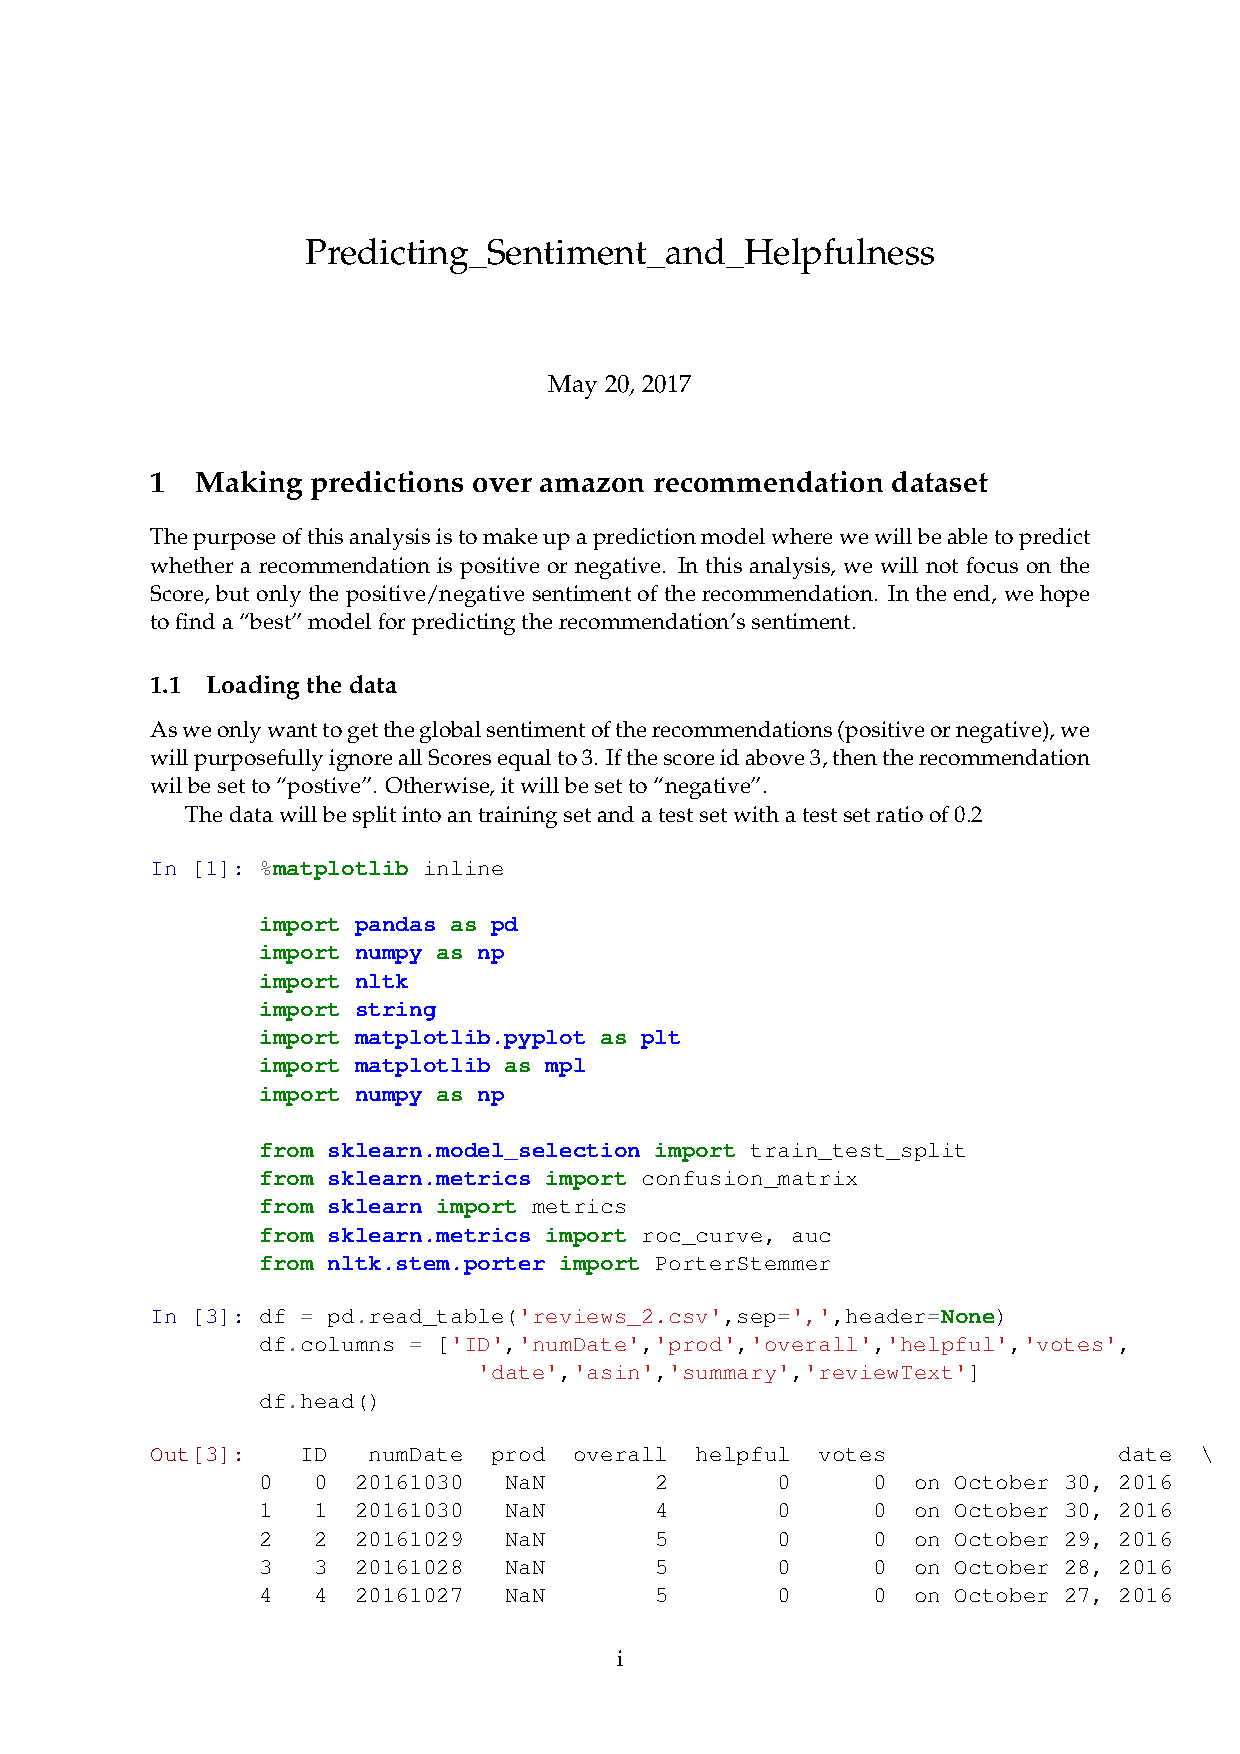
\includepdf[pages=-	,scale=1,pagecommand={\label{Predicting_Sentiment_and_Helpfulness}}]{pdf/Predicting_Sentiment_and_Helpfulness/Predicting_Sentiment_and_Helpfulness.pdf}

\invisiblesection{Topic Modeling}
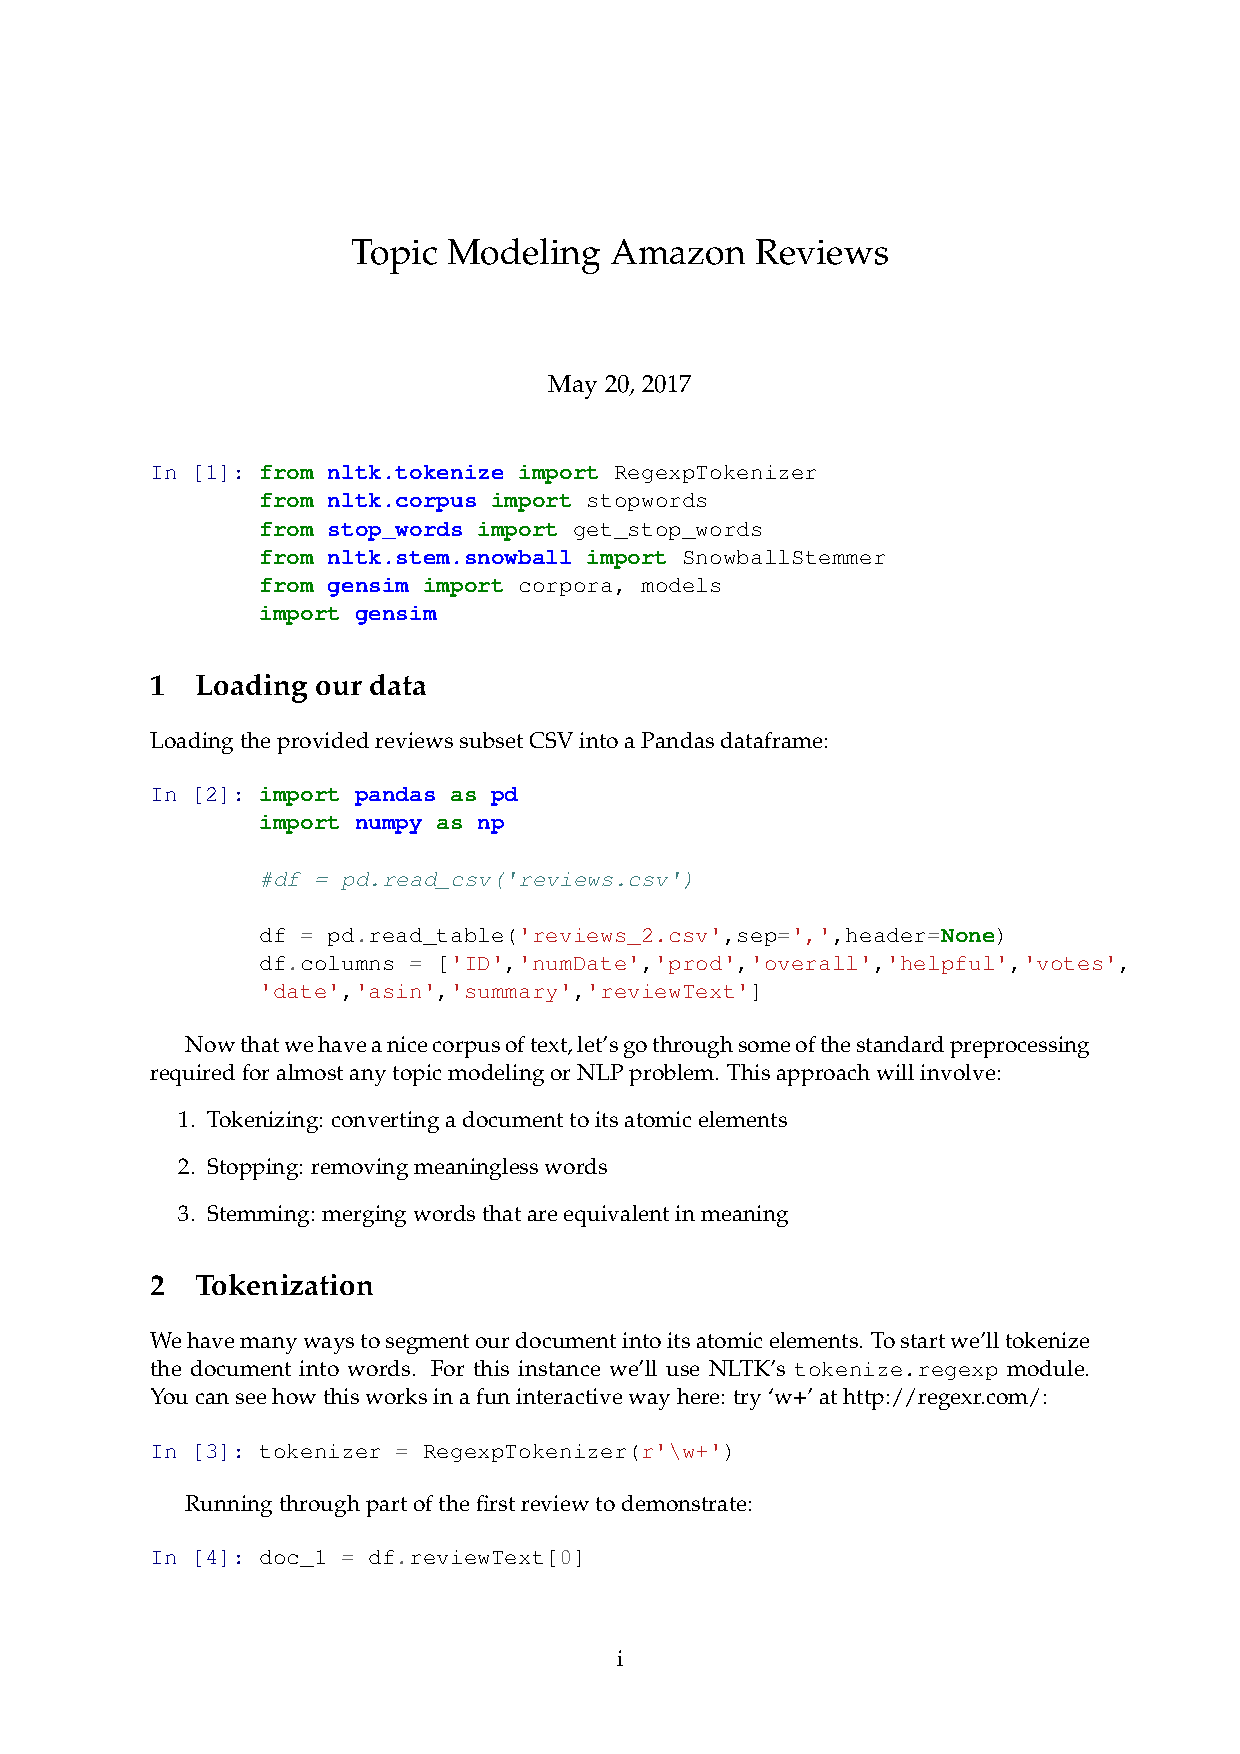
\includepdf[pages=-	,scale=1,pagecommand={\label{Topic_Modeling_Amazon_Reviews}}]{pdf/Topic/Topic_Modeling_Amazon_Reviews.pdf}

\invisiblesection{WordCloud Creation}
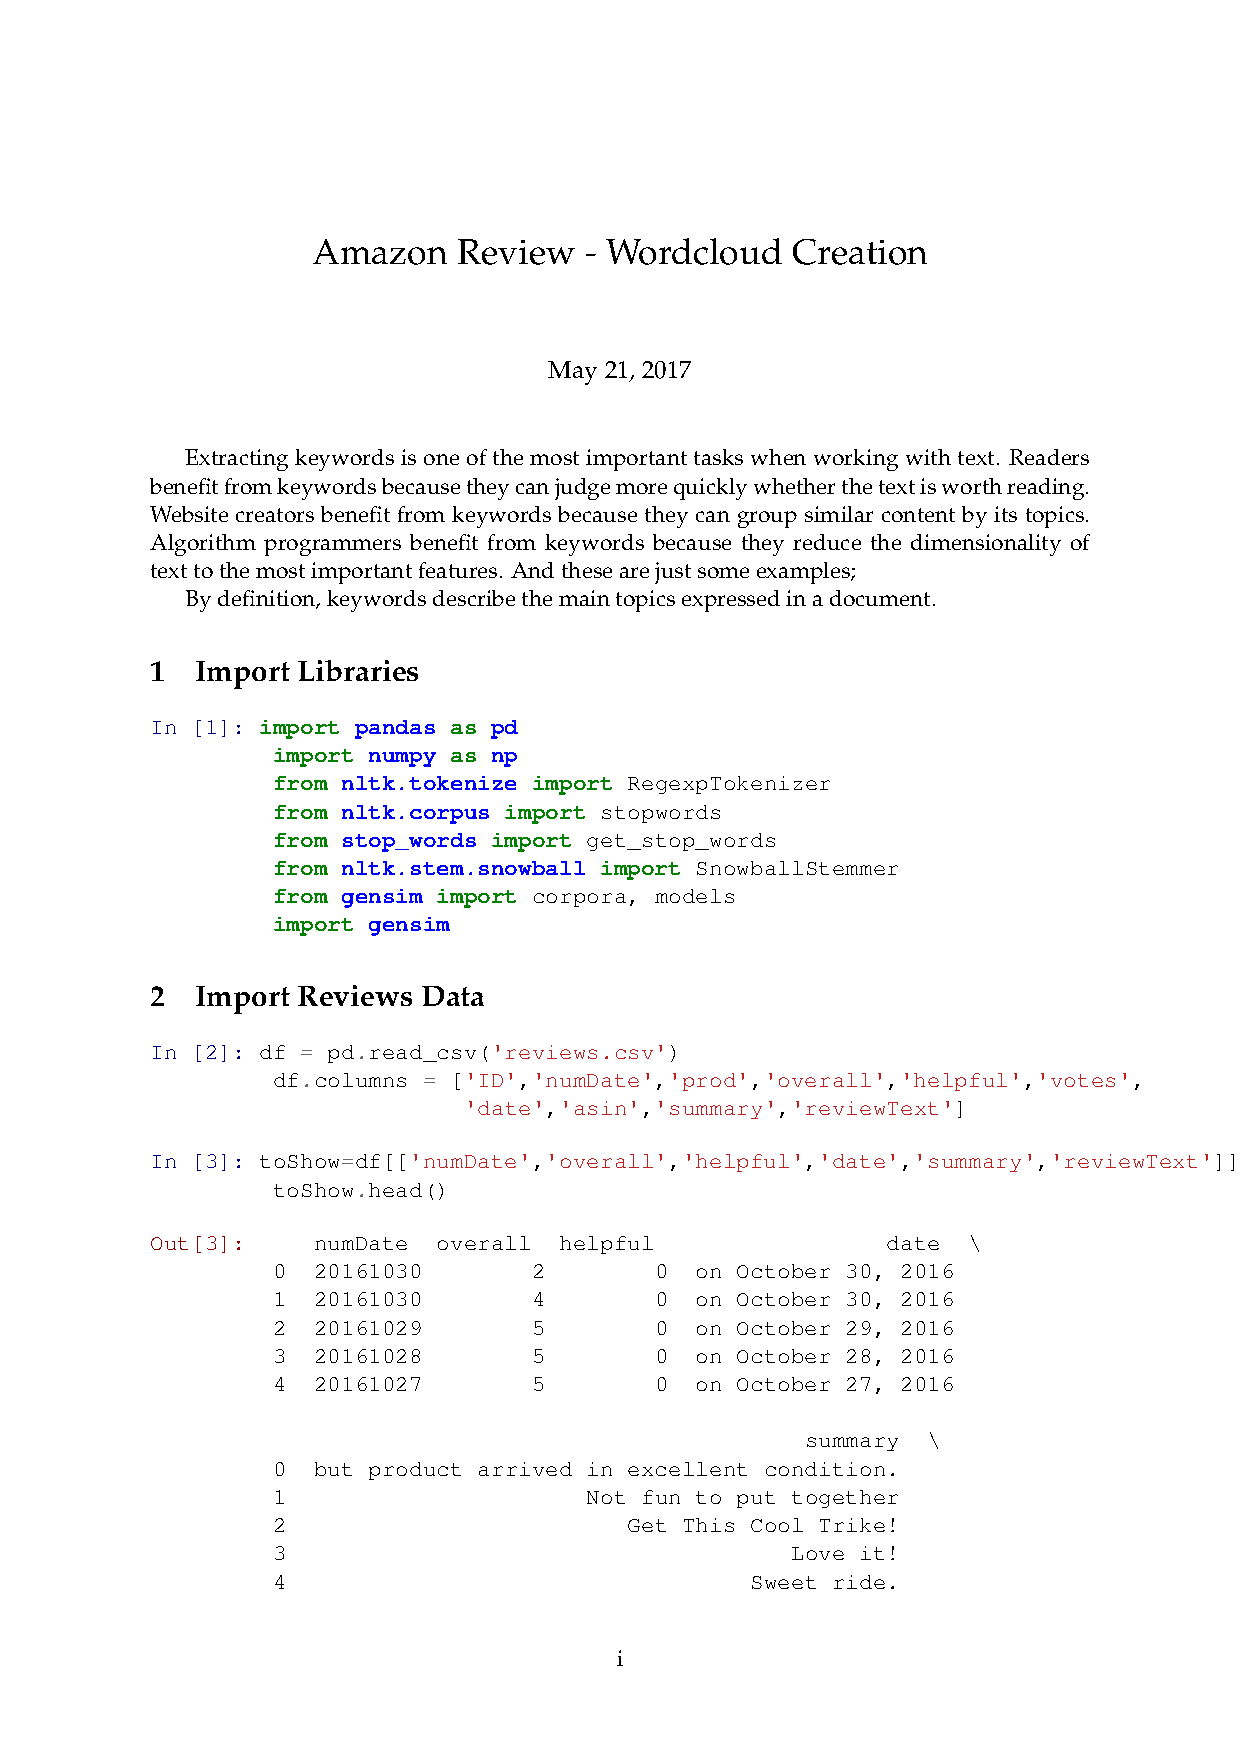
\includepdf[pages=-	,scale=1,pagecommand={\label{Amazon}}]{pdf/Amazon/Amazon.pdf}

\chapter{Arduino Code}
\textit{miniPEV - Arduino UNO} \\[10pt]
\textit{PEV - Arduino MEGA A} \\[10pt]
\textit{PEV - Arduino MEGA B}\\[10pt]

\newpage
\section{miniPEV - Arduino UNO}
\begin{lstlisting}[style=codearduino]
#include <Wire.h>
#include <Adafruit_Sensor.h>
#include <Adafruit_BNO055.h>
#include <utility/imumaths.h>
#include <Servo.h>
#include <Math.h>

Adafruit_BNO055 bno = Adafruit_BNO055();
Servo myServo1;
Servo myServo2;
int pinS1 = 10;
int pinS2 = 11;

int pinPot = 0;
int pot = 0;

int transistorPin = 3;
int V = 15;

float g = 9.81;
float phi_des = 0;
int delta = 0;
int t1 = 0;
int t2 = 0;

int led = 8;
int threshold = 150;
int deadband = 10;

int buttonPin = 2;         // the number of the input pin

int state = LOW;      // the current state of the output pin
int reading;           // the current reading from the input pin
int previous = HIGH;    // the previous reading from the input pin
long time = 0;         // the last time the output pin was toggled
long debounce = 200;   // the debounce time, increase if the output flickers

int ang_dev = 70;
const float pi = 3.1415;

const int numReadings = 25;
int readings1[numReadings];      // the readings from the analog input
int readIndex1 = 0;              // the index of the current reading
int total1 = 0;                  // the running total
int average1 = 0;                // the average

float readings2[numReadings];      // the readings from the analog input
int readIndex2 = 0;              // the index of the current reading
float total2 = 0;                  // the running total
float average2 = 0;                // the average

char val;
int pos = LOW;

void setup()
{
  Serial.begin(115200);

  myServo1.attach(pinS1);  myServo1.write(90);
  myServo2.attach(pinS2);  myServo2.write(ang_dev);
  if (!bno.begin())
  {
    Serial.print("Ooops, no BNO055 detected ... Check your wiring or I2C ADDR!");
    while (1);
  }
  //TIMSK0 = 0;
  for (int thisReading1 = 0; thisReading1 < numReadings; thisReading1++) {
    readings1[thisReading1] = 0;
  }
  for (int thisReading2 = 0; thisReading2 < numReadings; thisReading2++) {
    readings2[thisReading2] = 0;
  }

  bno.setExtCrystalUse(true);

  pinMode(buttonPin, INPUT);
  pinMode(led, OUTPUT);
  pinMode(transistorPin, OUTPUT);

  delay(1000);
}

void loop()
{

  reading = digitalRead(buttonPin);

  if (reading == HIGH && previous == LOW && millis() - time > debounce) {
    if (state == HIGH)
      state = LOW;
    else
      state = HIGH;

    time = millis();
  }

  digitalWrite(transistorPin, state);
  digitalWrite(led, state);
  previous = reading;

  total1 = total1 - readings1[readIndex1];
  readings1[readIndex1] = analogRead(pinPot);
  total1 = total1 + readings1[readIndex1];
  readIndex1 = readIndex1 + 1;
  if (readIndex1 >= numReadings) {
    readIndex1 = 0;
  }
  average1 = total1 / numReadings;

  pot = average1; //leer valor pot [0-1023]
  delta = map(pot, 0, 1023, 0, 180); //valor pot [0 - 180]
  myServo1.write(delta);

  sensors_event_t event;
  bno.getEventGyroscope(&event);

  total2 = total2 - readings2[readIndex2];
  readings2[readIndex2] = event.gyro.z;
  total2 = total2 + readings2[readIndex2];
  readIndex2 = readIndex2 + 1;
  if (readIndex2 >= numReadings) {
    readIndex2 = 0;
  }
  average2 = total2 / numReadings;

  phi_des = atan(average2 * V / g) * 180 / pi;
  //Serial.println(phi_des);
  myServo2.write(phi_des + ang_dev);
  delay(50);

  //Read input from bluetooth module:
  if ( Serial.available())
  {
    val = Serial.read();
  
    //Input key switch
    switch (val) {
    case '0':
      //Code when no key is pressed
      break;
    case '1':
      pos = HIGH;
      digitalWrite(led, pos);
      Serial.println("Case 1");
      //Code when UP key is pressed
      break;
    case '2':
      pos = LOW;
      digitalWrite(led, pos);
      Serial.println("Case 2");
      //Code when DOWN key is pressed
      break;
    case '3':
      //Code when LEFT key is pressed
      break;
    case '4':
      //Code when RIGHT key is pressed
      break;
    default:
      // default code (should never run)
      break;
    }
  }
}
\end{lstlisting}

\newpage
\section{PEV - Arduino MEGA A}
\begin{lstlisting}[style=codearduino]
// Arduino Mega for Three Nidec Motors (Tilt, Steer, Handle) & Bluetooth Remote Controller (HC06)

#include "VescUart.h"
#include "datatypes.h"
#include <Wire.h>
#include <Average.h>
#include <SoftwareSerial.h>
#include "I2C_Anything.h"

//Serial: 0-Debug 2-Tilting 1-Steering 3-Handle Bar
int tilt = 2, steer = 1, handle = 3;
const float pi = 3.1415;
#define DEBUG

float delta = 0.0, delta_prev = 0.0, delta2 = 0.0;
float delta_offset = 0, tilt_offset = 0, steer_offset = 0;
int flag1 = 0, flag2 = 0, flag3 = 0, flag4 = 0, flag5 = 0, flag6 = 0;
long tachometer_offset = 0;
struct bldcMeasure handle_bar;
int power_steer = 0;

SoftwareSerial btSerial(10, 11); // RX, TX
char bluetooth = '0';
int remote = 0, btread, demo = 0;

float delta_bt_prev = 0.0, delta_bt = 0.0, theta_bt = 0.0;
volatile boolean haveData = false;
volatile float M_t, delta_imu, theta_imu;

void setup() {
  // SERIAL ----------------------------------
  btSerial.begin(9600);  //BlueTooth
  Serial1.begin(115200); //Tilt
  Serial2.begin(115200); //Steer
  Serial3.begin(115200); //Handle
#ifdef DEBUG
  Serial.begin(115200);
#endif

  // WIRE I2C ---------------------------------
  Wire.begin(8);                // join i2c bus with address #8
  Wire.onReceive(receiveEvent); // register event
  Wire.onRequest(requestEvent); // register event


  // TO DO: INITIAL SETUP----------------------
  while (haveData)
  {
    Serial.print(M_t); Serial.print('\t');
    Serial.print(delta_imu); Serial.print('\t');
    Serial.print(theta_imu); Serial.print('\t');
    delta_offset = delta_imu;
    tilt_offset = theta_imu;
    haveData = false;
  }

  //  VescUartSetPosition(delta_offset, handle);
  //  delay(2000);
  //  if (VescUartGetValue(handle_bar, handle)) {
  //    tachometer_offset = handle_bar.tachometer;
  //  }

  // ------------------------------------------
}

long prev_time = 0;

void loop() {

  // HANDLE BAR HAPTIC FEEDBACK ----------------
  if (!remote) {
    handle_haptic(0);
    remote = 0;
  }

  // TILTING AND STEERING WITH MASTER DATA
  if (haveData)
  {
    Serial.print(M_t); Serial.print('\t');
    Serial.print(delta_bt); Serial.print('\t');
    Serial.print(delta_imu); Serial.print('\t');
    Serial.print(demo); Serial.print('\t');

    Serial.println(theta_imu); //Serial.print('\t');
    haveData = false;
    // TILTING MOTOR INPUT (I OR ANGLE) -----------
    float I = 0.5 + (M_t / 144) * 33 / 2;
    I = max(I, -5);
    I = min(I, 5);
    if(abs(theta_imu)<0.25){
      VescUartSetCurrent(-I, tilt); //if remote mode, put negative current (-I)
    }

    if(abs(theta_imu)>0.05 && abs(M_t)<5)
    {
      VescUartSetPosition(0, tilt);
    }

    // STEERING MOTOR ANGLE FROM HANDLE BAR INPUT (OR IMU) ----------
    //Serial.print(delta_imu); Serial.print('\t');
    if (!remote) {
      if (fabs(delta_imu) > 0.05 && fabs(delta_imu) < 0.5) {
        VescUartSetPosition(-delta_imu * 180 / pi, steer);
      }
    }

  }
  // BLUETOOTH COMMUNICATION -------------------
  //if (remote) {
    if ( btSerial.available())
    {
      remote = 1;
      btread = 1;
      bluetooth = btSerial.read();

      switch (bluetooth) {
        case '0':
          //Code when no key is pressed
          //VescUartSetCurrentBrake(0,steer);
          break;
        case '1':
          //Code when UP key is pressed
          break;
        case '2':
          //Code when DOWN key is pressed
          break;
        case '3':
          //Code when LEFT key is pressed
          if (power_steer) {
            delta_bt = delta_bt - 10;
          }
          break;
        case '4':
          //Code when RIGHT key is pressed
          if (power_steer) {
            delta_bt = delta_bt + 10;
          }
          break;
        case '5':
          //Code when SELECT key is pressed
          if (power_steer == 0) {
            power_steer = 1;
            delta_bt = 0;
          }
          else {
            power_steer = 0;
            VescUartSetCurrentBrake(3, steer);
          }
          break;
        case '6':
          //Code when START key is pressed
          break;
        case '7':
          //Code when SQUARE key is pressed
          theta_bt = theta_bt + 15;
          theta_bt = min(theta_bt, 60);
          VescUartSetPosition(theta_bt, tilt);
          break;
        case '8':
          //Code when TRIANGLE key is pressed
          // VescUartSetPosition(delta_bt, steer);
          // Include flag for Sponsors Week Demo
          if(demo==0){
            demo=1;
          }
          else{
            demo=0;
          }
          break;
        case '9':
          //Code when X key is pressed
          theta_bt = theta_bt - 15;
          theta_bt = max(theta_bt, -60);
          VescUartSetPosition(theta_bt, tilt);
          break;
        case 'A':
          //Code when CIRCLE key is pressed
          // BACK TO INITIAL STATE
          VescUartSetPosition(delta_offset, handle);
          VescUartSetPosition(tilt_offset, tilt);
          VescUartSetPosition(steer_offset, steer);
          delay(1000);
          // INITIAL OFFSET UPDATE
          delta_offset = delta_imu;
          tilt_offset = theta_imu;
          steer_offset = 0;
          delta_bt = 0;
          break;
        default:
          break;
      }

    //}
    delta_bt = max(delta_bt, -40);
    delta_bt = min(delta_bt, 40);
    if (delta_bt_prev != delta_bt) {
      VescUartSetPosition(delta_bt, steer);
      VescUartSetPosition(-delta_bt, handle);
    }
    delta_bt_prev = delta_bt;
  }
  //Serial.println();

  prev_time = millis();
}

// READ DATA FROM MASTER ARDUINO 2 -----------
void receiveEvent(int howMany) {
  if (howMany >= (sizeof M_t) + (sizeof delta_imu) + (sizeof theta_imu))
  {
    I2C_readAnything (M_t);
    I2C_readAnything (delta_imu);
    I2C_readAnything (theta_imu);
    haveData = true;
  }
}

// SEND DATA TO MASTER ARDUINO 2 --------------
void requestEvent() {
  if (remote && btread) {
    Wire.write(bluetooth); // respond with message of 1 bytes as expected by master
    btread = 0;
  }
}

void handle_haptic(int show) {

  //tachometer_offset = handle_bar.tachometer;
  if (VescUartGetValue(handle_bar, handle)) {

    delta = float(handle_bar.tachometer - tachometer_offset) / 17.47; //Change 17.47 for tachometer formulae
    if (abs(handle_bar.rpm) > 10) {
      delta2 = delta2 + float(handle_bar.rpm) / 60 * 360 / 1152 * float(millis() - prev_time) / 1000;
    }
    // delta3=Euler IMU A

    if (show) {
      Serial.print(float(handle_bar.tachometer - tachometer_offset)); Serial.print('\t');
      Serial.print(handle_bar.dutyCycleNow); Serial.print('\t');
      Serial.print(handle_bar.avgMotorCurrent); Serial.print('\t');
      Serial.print(handle_bar.avgInputCurrent); Serial.print('\t');
      Serial.print(handle_bar.rpm); Serial.print('\t');
      Serial.print(handle_bar.inpVoltage); Serial.print('\t');
      Serial.print(millis()); Serial.print('\t');
      Serial.print(flag1); Serial.print('\t');
      Serial.print(flag2); Serial.print('\t');
      Serial.print(flag3); Serial.print('\t');
      Serial.print(flag4); Serial.print('\t');
      Serial.print(flag5); Serial.print('\t');
      Serial.print(flag6); Serial.print('\t');
      Serial.print(delta); Serial.print('\t');
      Serial.println(delta2);
    }
    float delta_trans = 5;
    float delta_limit = 30;
    float delta_top = 50;

    // Return to center if excessive delta
    if (delta > delta_top) {
      flag5 = 1; flag3 = 0; flag1 = 0;
      VescUartSetPosition(0.0, handle);
    }
    else if (flag5 == 1 && abs(float(delta - delta_prev)) == 0) {
      flag5 = 0;
      tachometer_offset = handle_bar.tachometer;
    }
    // Return to center if excessive delta
    if (delta < -delta_top) {
      flag6 = 1; flag4 = 0; flag2 = 0;
      VescUartSetPosition(0.0, handle);
    }
    else if (flag6 == 1 && abs(float(delta - delta_prev)) == 0) {
      flag6 = 0;
      tachometer_offset = handle_bar.tachometer;
    }

    if (flag5 == 0)
    {
      //CW Limit Zone
      if (flag3 == 1 && handle_bar.avgMotorCurrent < 0.25 && handle_bar.rpm > 15)
      {
        VescUartSetDuty(0.00, handle);
      }
      else if (delta > delta_limit && handle_bar.rpm > 150 && flag3 == 0 )//&& (handle_bar.avgMotorCurrent == 0.0 || flag1 == 1))
      {
        VescUartSetDuty(0.00, handle);
        flag3 = 1;
      }
      else if (flag3 == 1 && (handle_bar.avgMotorCurrent > 0.45 || handle_bar.rpm < 0))
      {
        VescUartSetCurrentBrake(0.0, handle);
        flag3 = 0;
      }
      else if (flag3 == 1 && handle_bar.rpm < 50)
      {
        VescUartSetCurrentBrake(0.0, handle);
      }
    }
    if (flag6 == 0)
    {
      //CCW Limit Zone
      if (flag4 == 1 && handle_bar.avgMotorCurrent > 0.0 && handle_bar.rpm < 50)
      {
        VescUartSetDuty(0.00, handle);
      }
      else if (delta < -delta_limit && handle_bar.rpm < -200 && flag4 == 0 && (handle_bar.avgMotorCurrent == 0.0 || flag2 == 1))
      {
        VescUartSetDuty(0.00, handle);
        flag4 = 1;
      }
      else if (flag4 == 1 && ((handle_bar.avgMotorCurrent < -0.1 && handle_bar.rpm > 100) || handle_bar.rpm > 300))
      {
        VescUartSetCurrentBrake(0.0, handle);
        flag4 = 0;
      }
    }
    if (flag3 == 0)
    {
      
    }
    if (flag3 == 0 && flag4 == 0 && flag5 == 0 && flag6 == 0)
    {
      if (abs(delta) > delta_trans && abs(delta) < delta_limit && handle_bar.rpm > 150 ) {
        float duty = (delta_limit - delta) / (delta_limit - delta_trans);
        duty = max(duty, 0); duty = min(duty, 1); int T;
        if (duty < 0.02) {
          T = 1000;
        }
        else {
          T = duty * 1000;
        }
        VescUartSetDuty(duty, handle);
        delayMicroseconds(T);
        VescUartSetDuty(-duty, handle);
        delayMicroseconds(1);
        VescUartSetCurrentBrake(0.0, handle);
      }
      else if (abs(delta) > delta_trans && abs(delta) < delta_limit && handle_bar.rpm < -150 ) {
        float duty = (delta_limit - delta) / (delta_limit - delta_trans);
        duty = max(duty, 0); duty = min(duty, 1); int T;
        if (duty < 0.02) {
          T = 1000;
        }
        else {
          T = duty * 1000;
        }

        VescUartSetDuty(-duty, handle);
        delayMicroseconds(T);
        VescUartSetDuty(duty, handle);
        delayMicroseconds(1);
        VescUartSetCurrentBrake(0.0, handle);
      }
      //else if (delta > delta_trans && abs(handle_bar.rpm) < 150) {  VescUartSetPosition(0.0,handle);  }
    }
    if (flag4 == 0)
    {
      
    }
    //Restart variables only if we read
    delta_prev = delta;
    prev_time = millis();
  }
  else  {
    Serial.println("Failed to get data from Handle Bar!");
  }
}
void vibrate_A() {
  prev_time = micros();
  while ((micros() - prev_time) < 750000)
  {
    float duty = 0.5;
    VescUartSetDuty(duty, handle);
    delayMicroseconds(10000);
    VescUartSetDuty(-duty, handle);
    delayMicroseconds(10000);
  }
  VescUartSetCurrentBrake(0.0, handle);
  //delay(2000);
}
void vibrate_B() {
  prev_time = micros();
  while ((micros() - prev_time) < 750000)
  {
    float duty = 1; //0.4
    VescUartSetDuty(duty, handle);
    delayMicroseconds(20000); //7000
    VescUartSetDuty(-duty, handle);
    delayMicroseconds(20000);
  }
  VescUartSetCurrentBrake(0.0, handle);
  //delay(2000);
}


\end{lstlisting}

\newpage
\section{PEV - Arduino MEGA B}
\begin{lstlisting}[style=codearduino]
// Arduino Mega for IMU_A, IMU_B, Throttle, Encoder, Rear Motor & Processing Serial Export (HC05)

#include "VescUart.h"
#include "datatypes.h"
#include <Average.h>
#include <digitalWriteFast.h>
#include <Wire.h>
#include <Adafruit_Sensor.h>
#include <Adafruit_BNO055.h>
#include <utility/imumaths.h>
#include <Math.h>
#include "I2C_Anything.h"
#include <SoftwareSerial.h>
SoftwareSerial btSerial(10, 11); // RX, TX
#define DEBUG

#define c_EncoderInterrupt 0
#define c_EncoderPinA 3
#define c_EncoderPinB 2
#define EncoderIsReversed
volatile bool _EncoderBSet;
volatile long _EncoderTicks = 0;
volatile long _EncoderTicks_prev = 0;
float rear_radius = 24.25e-3, v = 0.0;
const float pi = 3.1415;

int processing = 1, calibration_IMU_A = 0, calibration_initial_IMU_A = 0, calibration_IMU_B = 0, calibration_initial_IMU_B = 0;
int print_IMU_A = 0, print_IMU_B = 0, print_control = 1 , print_throttle = 0, print_encoder = 1;
int rear = 1, throttlePin = 0, pot_min = 248, pot_max = 798;
float rear_duty = 0, bt_duty = 0, theta_offset = -0.11 , delta_offset = -2.49, power_rear = 0.0;
char bluetooth;

Average<float> aper(5);
Average<float> thita(5);

// The two BNO055 modules, bnoB has the ADR pin wired to 3.3v to change its i2c address
// Both are wired: SCL to analog 5, SDA to analog 4, VIN to 5v, GRN to ground
Adafruit_BNO055 bnoA = Adafruit_BNO055(-1, BNO055_ADDRESS_A);
Adafruit_BNO055 bnoB = Adafruit_BNO055(-1, BNO055_ADDRESS_B);


typedef struct {
  double q; //process noise covariance
  double r; //measurement noise covariance
  double x; //value
  double p; //estimation error covariance
  double k; //kalman gain
} kalman_state;

double p = 1, q = 0.02, r = 0.15, x = 0, measurement, k;
kalman_state v_k, a_per_k, phi_p_k, theta_k, theta_p_k, a_per_i_k, delta_k, delta_p_k;


void setup() {
  // SERIAL ----------------------------------
  btSerial.begin(115200);  //BlueTooth
  Serial1.begin(115200); // Rear Motor
#ifdef DEBUG
  Serial.begin(115200);  // Debug
#endif

  // ENCODER ---------------------------------
  pinMode(c_EncoderPinA, INPUT);      // sets pin A as input
  digitalWrite(c_EncoderPinA, LOW);  // turn on pullup resistors
  pinMode(c_EncoderPinB, INPUT);      // sets pin B as input
  digitalWrite(c_EncoderPinB, LOW);  // turn on pullup resistors
  attachInterrupt(c_EncoderInterrupt, HandleMotorInterruptA, RISING);

  // THROTTLE ---------------------------------
  pinMode(throttlePin, INPUT);
  digitalWrite(throttlePin, LOW);
  pinMode(13, OUTPUT);

  // IMUs CALIBRATION -------------------------
  Wire.begin();

  // IMU A ------------------------------------
  bnoA.begin();
  bnoA.setMode(0X00);
  bnoA.setAccelRange();
  const adafruit_bno055_offsets_t &offsets_type_A = {65526, 65527, 30, 65535, 65535, 0, 65437, 157, 114, 1000, 0};
  //const adafruit_bno055_offsets_t &offsets_type_A = {65526,65527,30,65534,65535,0,65437,157,114,1000,0};

  bnoA.setSensorOffsets(offsets_type_A);
  bnoA.setMode(0X0C);

  if (calibration_IMU_A) {
    while (!bnoA.isFullyCalibrated())
    {
      uint8_t system, gyro, accel, mag = 0;
      bnoA.getCalibration(&system, &gyro, &accel, &mag);
      Serial.print("CALIBRATION A: Sys=");    Serial.print(system, DEC);
      Serial.print(" Gyro=");    Serial.print(gyro, DEC);
      Serial.print(" Accel=");   Serial.print(accel, DEC);
      Serial.print(" Mag=");     Serial.println(mag, DEC);

      if (calibration_initial_IMU_A) {
        adafruit_bno055_offsets_t offsets_type_A_2;
        if (bnoA.getSensorOffsetsAlways(offsets_type_A_2))
        {
          Serial.print(offsets_type_A_2.accel_offset_x);    Serial.print(",");
          Serial.print(offsets_type_A_2.accel_offset_y);    Serial.print(",");
          Serial.print(offsets_type_A_2.accel_offset_z);    Serial.print(",");
          Serial.print(offsets_type_A_2.gyro_offset_x);    Serial.print(",");
          Serial.print(offsets_type_A_2.gyro_offset_y);    Serial.print(",");
          Serial.print(offsets_type_A_2.gyro_offset_z);    Serial.print(",");
          Serial.print(offsets_type_A_2.mag_offset_x);    Serial.print(",");
          Serial.print(offsets_type_A_2.mag_offset_y);    Serial.print(",");
          Serial.print(offsets_type_A_2.mag_offset_z);    Serial.print(",");
          Serial.print(offsets_type_A_2.accel_radius);    Serial.print(",");
          Serial.println(offsets_type_A_2.mag_radius);
        }
      }
    }
    uint8_t system, gyro, accel, mag = 0;
    bnoA.getCalibration(&system, &gyro, &accel, &mag);
    Serial.print("CALIBRATION A: Sys=");    Serial.print(system, DEC);
    Serial.print(" Gyro=");    Serial.print(gyro, DEC);
    Serial.print(" Accel=");   Serial.print(accel, DEC);
    Serial.print(" Mag=");     Serial.println(mag, DEC);
  }

  // IMU B ----------------------------------------
  bnoB.begin();
  bnoB.setMode(0X00);
  bnoB.setAccelRange();
  //const adafruit_bno055_offsets_t &offsets_type_B = {65526, 65527, 30, 65535, 65535, 0, 65437, 157, 114, 1000, 0};//867
  //const adafruit_bno055_offsets_t &offsets_type_B = {11,4,21,1,1,65535,65437,157,114,1000,0};
  const adafruit_bno055_offsets_t &offsets_type_B = {65528, 65528, 17, 0, 0, 65535, 65406, 150, 114, 1000, 1200};
  bnoB.setSensorOffsets(offsets_type_B);
  bnoB.setMode(0X0C);

  if (calibration_IMU_B) {
    while (!bnoB.isFullyCalibrated())
    {
      uint8_t system, gyro, accel, mag = 0;
      bnoB.getCalibration(&system, &gyro, &accel, &mag);
      Serial.print("CALIBRATION B: Sys=");    Serial.print(system, DEC);
      Serial.print(" Gyro=");    Serial.print(gyro, DEC);
      Serial.print(" Accel=");   Serial.print(accel, DEC);
      Serial.print(" Mag=");     Serial.println(mag, DEC);

      if (calibration_initial_IMU_B) {
        adafruit_bno055_offsets_t offsets_type_B_2;
        if (bnoB.getSensorOffsetsAlways(offsets_type_B_2))
        {
          Serial.print(offsets_type_B_2.accel_offset_x);    Serial.print(",");
          Serial.print(offsets_type_B_2.accel_offset_y);    Serial.print(",");
          Serial.print(offsets_type_B_2.accel_offset_z);    Serial.print(",");
          Serial.print(offsets_type_B_2.gyro_offset_x);    Serial.print(",");
          Serial.print(offsets_type_B_2.gyro_offset_y);    Serial.print(",");
          Serial.print(offsets_type_B_2.gyro_offset_z);    Serial.print(",");
          Serial.print(offsets_type_B_2.mag_offset_x);    Serial.print(",");
          Serial.print(offsets_type_B_2.mag_offset_y);    Serial.print(",");
          Serial.print(offsets_type_B_2.mag_offset_z);    Serial.print(",");
          Serial.print(offsets_type_B_2.accel_radius);    Serial.print(",");
          Serial.println(offsets_type_B_2.mag_radius);
        }
      }
    }
    uint8_t system, gyro, accel, mag = 0;
    bnoB.getCalibration(&system, &gyro, &accel, &mag);
    Serial.print("CALIBRATION B: Sys=");    Serial.print(system, DEC);
    Serial.print(" Gyro=");    Serial.print(gyro, DEC);
    Serial.print(" Accel=");   Serial.print(accel, DEC);
    Serial.print(" Mag=");     Serial.println(mag, DEC);
  }

  // EXPORT PROCESSING DATA -----------------------------
  if (processing) {
    //    btSerial.println("CLEARDATA"); //clears up any data left from previous projects
    //    btSerial.println("LABEL,..."); //always write LABEL, so excel knows the next things will be the names of the columns (instead of Acolumn you could write Time for instance)
    //    btSerial.println("RESETTIMER"); //resets timer to 0
  }

  // Calculate initial angle offsets

  // IMU_A DATA -------------------------------------
  imu::Quaternion quat_A = bnoA.getQuat();
  double resA[3];
  //char RotSeq[12]=[zyx, zyz, zxy, zxz, yxz, yxy, yzx, yzy, xyz, xyx, xzy, xzx];
  imu::Vector<3> eulerYZX_A = quat_A.quaternion2Euler(7, resA);
  delay(1000);
  // IMU_B DATA ------------------------------------- eulerXZY_B.y()
  imu::Quaternion quat_B = bnoB.getQuat();
  double resB[3];
  //char RotSeq[12]=[zyx, zyz, zxy, zxz, yxz, yxy, yzx, yzy, xyz, xyx, xzy, xzx];
  imu::Vector<3> eulerXZY_B = quat_B.quaternion2Euler(1, resB);

  theta_offset = eulerXZY_B.y();
  delta_offset = eulerYZX_A.x() - eulerXZY_B.z();
  Wire.beginTransmission(8); // transmit to device #8
  I2C_writeAnything (0.0);
  I2C_writeAnything (delta_offset - delta_offset);
  I2C_writeAnything (theta_offset - theta_offset);
  Wire.endTransmission();    // stop transmitting
  // -------------------------------------------
  float eulerYZX_A_x_prev = eulerYZX_A.x(), eulerXZY_B_z_prev = eulerXZY_B.z();
  Serial.print(eulerYZX_A.x());  Serial.print('\t');
  Serial.print(eulerXZY_B.z());  Serial.print('\t');
  Serial.print(theta_offset);  Serial.print('\t');
  Serial.print(delta_offset);  Serial.print('\t');

  // KALMAN INITIALIZATION
  v_k = kalman_init(0.005, 0.05, p, x);
  a_per_k = kalman_init(0.01, 0.15, p, x);
  phi_p_k = kalman_init(0.1, r, p, x);
  theta_k = kalman_init(q, r, p, x);
  theta_p_k = kalman_init(q, r, p, x);
  a_per_i_k = kalman_init(q, r, p, x);
  delta_k = kalman_init(q, r, p, x);
  delta_p_k = kalman_init(q, r, p, x);

  digitalWrite(13, HIGH);
  delay(1000);
  digitalWrite(13, LOW);
}
float eulerXZY_B_z, eulerYZX_A_x, eulerYZX_A_x_prev = 0, eulerXZY_B_z_prev = 0, vel = 0.0;
int k_A = 0, k_B = 0;
long delay_loop = 0;
float prev_time = 0, prev_time_enc = micros(), prev_time_a_per = micros();

// GAINS WITHOUT DRIVER AND INVERSE TERM
float k_a_per_c = -0.31, k_phi_p_c = 11.11, k_theta_c = 249.12, k_theta_p_c = 65.51, k_a_per_i_c = -1.00, k_delta_c = 686.17, k_delta_p_c = 123.24;
float k_a_per_v = -0.29, k_phi_p_v = -3.62, k_theta_v = -2.72, k_theta_p_v = -0.49, k_a_per_i_v = 0.00, k_delta_v = -239.04, k_delta_p_v = -54.16;
float k_a_per_v_inv = 0, k_phi_p_v_inv = 0, k_theta_v_inv = 0, k_theta_p_v_inv = 0, k_a_per_i_v_inv = 0.00, k_delta_v_inv = 0, k_delta_p_v_inv = 0;

float a_per, a_per_prev = 0, phi_p , theta , theta_p , a_per_i = 0.0 , delta , delta_p ;

void loop() {

  // ROTARY ENCODER VELOCITY ------------------------

  v = float(_EncoderTicks - _EncoderTicks_prev) / (float(micros() - prev_time_enc) / 1000000) / 1000.0 * 2 * pi * rear_radius; // replace 20 for real delay
  if (fabs(v) < 0.1) {
    v = 0.0;
  }
  kalman_update(&v_k, v);
  if (print_encoder) {
    Serial.print(v_k.x);   Serial.print('\t');
  }
  _EncoderTicks_prev = _EncoderTicks;
  prev_time_enc = micros();
  //delay(20);

  //  IMU -------------------------------------------
  //  VECTOR_ACCELEROMETER - m/s^2
  //  VECTOR_MAGNETOMETER  - uT
  //  VECTOR_GYROSCOPE     - rad/s
  //  VECTOR_EULER         - degrees
  //  VECTOR_LINEARACCEL   - m/s^2
  //  VECTOR_GRAVITY       - m/s^2

  // IMU_A DATA -------------------------------------
  imu::Vector<3> linear_accel_A = bnoA.getVector(Adafruit_BNO055::VECTOR_LINEARACCEL);
  imu::Vector<3> gyro_A = bnoA.getVector(Adafruit_BNO055::VECTOR_GYROSCOPE);
  imu::Vector<3> euler_A = bnoA.getVector(Adafruit_BNO055::VECTOR_EULER);
  imu::Vector<3> accel_A = bnoA.getVector(Adafruit_BNO055::VECTOR_ACCELEROMETER);
  imu::Quaternion quat_A = bnoA.getQuat();
  double resA[3];
  //char RotSeq[12]=[zyx, zyz, zxy, zxz, yxz, yxy, yzx, yzy, xyz, xyx, xzy, xzx];
  imu::Vector<3> eulerYZX_A = quat_A.quaternion2Euler(7, resA);

  // Continuous angle
  if (eulerYZX_A_x_prev > pi / 2 && eulerYZX_A.x() < -pi / 2) {
    k_A = k_A + 1;
  }
  else if (eulerYZX_A_x_prev < -pi / 2 && eulerYZX_A.x() > pi / 2) {
    k_A = k_A - 1;
  }
  eulerYZX_A_x = eulerYZX_A.x() + k_A * 2 * pi;
  eulerYZX_A_x_prev = eulerYZX_A.x();

  if (print_IMU_A) {
    Serial.print(linear_accel_A.x()); Serial.print('\t');
    Serial.print(linear_accel_A.y()); Serial.print('\t');
    Serial.print(linear_accel_A.z()); Serial.print('\t');
    Serial.print(gyro_A.x()); Serial.print('\t');
    Serial.print(gyro_A.y()); Serial.print('\t');
    Serial.print(gyro_A.z()); Serial.print('\t');
    Serial.print(eulerYZX_A.x()); Serial.print('\t');
    Serial.print(eulerYZX_A.y()); Serial.print('\t');
    Serial.print(eulerYZX_A.z()); Serial.print('\t');
    Serial.print(euler_A.x()); Serial.print('\t');
    Serial.print(euler_A.y()); Serial.print('\t');
    Serial.print(euler_A.z()); Serial.print('\t');
    Serial.print(accel_A.x()); Serial.print('\t');
    Serial.print(accel_A.y()); Serial.print('\t');
    Serial.print(accel_A.z()); Serial.print('\t');
  }

  // IMU_B DATA -------------------------------------
  imu::Vector<3> linear_accel_B = bnoB.getVector(Adafruit_BNO055::VECTOR_LINEARACCEL);
  imu::Vector<3> gyro_B = bnoB.getVector(Adafruit_BNO055::VECTOR_GYROSCOPE);
  imu::Vector<3> euler_B = bnoB.getVector(Adafruit_BNO055::VECTOR_EULER);
  imu::Vector<3> accel_B = bnoB.getVector(Adafruit_BNO055::VECTOR_ACCELEROMETER);
  imu::Quaternion quat_B = bnoB.getQuat();
  double resB[3];
  //char RotSeq[12]=[zyx, zyz, zxy, zxz, yxz, yxy, yzx, yzy, xyz, xyx, xzy, xzx];
  imu::Vector<3> eulerXZY_B = quat_B.quaternion2Euler(1, resB);

  // Continuous angle
  if (eulerXZY_B_z_prev > pi / 2 && eulerXZY_B.z() < -pi / 2) {
    k_B = k_B + 1;
  }
  else if (eulerXZY_B_z_prev < -pi / 2 && eulerXZY_B.z() > pi / 2) {
    k_B = k_B - 1;
  }
  eulerXZY_B_z = eulerXZY_B.z() + k_B * 2 * pi;
  eulerXZY_B_z_prev = eulerXZY_B.z();
  if (print_IMU_B) {
    Serial.print(linear_accel_B.x()); Serial.print('\t');
    Serial.print(linear_accel_B.y()); Serial.print('\t');
    Serial.print(linear_accel_B.z()); Serial.print('\t');
    Serial.print(gyro_B.x()); Serial.print('\t');
    Serial.print(gyro_B.y()); Serial.print('\t');
    Serial.print(gyro_B.z()); Serial.print('\t');
    Serial.print(eulerXZY_B.x()); Serial.print('\t');
    Serial.print(eulerXZY_B.y()); Serial.print('\t');
    Serial.print(eulerXZY_B.z()); Serial.print('\t');
    Serial.print(euler_B.x()); Serial.print('\t');
    Serial.print(euler_B.y()); Serial.print('\t');
    Serial.print(euler_B.z()); Serial.print('\t');
    Serial.print(accel_B.x()); Serial.print('\t');
    Serial.print(accel_B.y()); Serial.print('\t');
    Serial.print(accel_B.z()); Serial.print('\t');
  }
  // THROTTLE VALUE ---------------------------------
  rear_duty = float(analogRead(throttlePin) - pot_min) / (pot_max - pot_min);
  if (print_throttle) {
    Serial.print(rear_duty); Serial.print('\t');
    Serial.print(analogRead(throttlePin)); Serial.print('\t');
  }
  // REAR MOTOR POWER ASSIST ------------------------
  if (rear_duty > 0.1 && rear_duty < 0.9) {
    VescUartSetDuty(rear_duty, rear);
  }
  else {
    VescUartSetCurrentBrake(0, rear);
  }
  // CONTROL CALCULATIONS -----------------------------------
  float delay_mili = (micros() - prev_time);
  // a_per Kalman Filter ------------------------------------
  if (fabs(linear_accel_B.x()) > 0.5) { //0.5
    kalman_update(&a_per_k, linear_accel_B.x());
  }
  else {
    kalman_update(&a_per_k, 0.0);
  }
  // a_per_i Integration + Kalman Filter-----------------------
  if (abs(a_per_k.x) > 0.02) {
    vel = vel + (micros() - prev_time) / 1000000 * a_per_k.x;
  }
  else {
    vel = 0;
  }
  kalman_update(&a_per_i_k, vel);
  // phi_p Kalman Filter   ----------------------------------
  if (fabs(gyro_B.y()) > 0.05) { //0.2
    kalman_update(&phi_p_k, gyro_B.y());
  }
  else {
    kalman_update(&phi_p_k, 0.0);
  }
  // theta Kalman Filter    ---------------------------------
  if (fabs(eulerXZY_B.y() - theta_offset) > 0.01) { //0.1
    kalman_update(&theta_k, eulerXZY_B.y() - theta_offset);
  }
  else {
    kalman_update(&theta_k, 0.0);
  }
  // theta_p Kalman Filter  ---------------------------------
  if (fabs(gyro_B.z()) > 0.05) { //0.2
    kalman_update(&theta_p_k, gyro_B.z());
  }
  else {
    kalman_update(&theta_p_k, 0.0);
  }
  // delta Kalman Filter   ----------------------------------
  if (fabs(eulerYZX_A_x - eulerXZY_B_z - delta_offset) > 0.05) { //0.2
    kalman_update(&delta_k, eulerYZX_A_x - eulerXZY_B_z - delta_offset);
  }
  else {
    kalman_update(&delta_k, 0.0);
  }
  // delta_p Kalman Filter ----------------------------------
  if (fabs(gyro_A.x()) > 0.05) { //0.2
    kalman_update(&delta_p_k, gyro_A.x());
  }
  else {
    kalman_update(&delta_p_k, 0.0);
  }

  a_per = a_per_k.x; // m/s^2
  phi_p = phi_p_k.x; // rad/s
  theta = theta_k.x; // rad
  theta_p = theta_p_k.x; // rad/s
  a_per_i = a_per_i_k.x; // m/s
  delta = delta_k.x; // rad eulerYZX_A.x() - eulerXZY_B.z();
  delta_p = delta_p_k.x; // rad/s

  a_per_prev = a_per;
  prev_time_a_per = micros();

  // FEEDBACK CONSTANTS CALCULATION = F(V)
  float V = v_k.x;
  float u;
  if (fabs(V) > 1) {
    u = -(k_a_per_c + k_a_per_v * V + k_a_per_v_inv / V) * a_per - (k_phi_p_c + k_phi_p_v * V + k_phi_p_v_inv / V) * phi_p - (k_theta_c + k_theta_v * V + k_theta_v_inv / V) * theta - (k_theta_p_c + k_theta_p_v * V + k_theta_p_v_inv / V) * theta_p - (k_a_per_i_c + k_a_per_i_v * V + k_a_per_i_v_inv / V) * a_per_i - (k_delta_c + k_delta_v * V + k_delta_v_inv / V) * delta - (k_delta_p_c + k_delta_p_v * V + k_delta_p_v_inv / V) * delta_p ;
  }
  else {
    u = -k_a_per_c * a_per - k_phi_p_c * phi_p - k_theta_c * theta - k_theta_p_c * theta_p - k_a_per_i_c * a_per_i - k_delta_c * delta - k_delta_p_c * delta_p;
    u = 0.00;
  }

  if (print_control) {
    //    Serial.print(eulerYZX_A.x()); Serial.print('\t');
    //    Serial.print(eulerXZY_B.z());  Serial.print('\t');
    
    Serial.print(a_per); Serial.print('\t');
    Serial.print(phi_p); Serial.print('\t');
    Serial.print(theta); Serial.print('\t');
    Serial.print(theta_p); Serial.print('\t');
    Serial.print(a_per_i); Serial.print('\t');
    Serial.print(delta); Serial.print('\t');
    Serial.print(delta_p); Serial.print('\t');
    Serial.print(delay_mili); Serial.print('\t');
    Serial.print(u); Serial.print('\t');
  }

  // SEND DATA TO SLAVE ARDUINO 1 -------------------
  Wire.beginTransmission(8); // transmit to device #8
  I2C_writeAnything (u);
  I2C_writeAnything (delta);
  I2C_writeAnything (theta);
  Wire.endTransmission();    // stop transmitting
  //delay(5);

  // RECEIVE DATA FROM SLAVE ARDUINO 1 --------------
  int nbytes = 1;
  Wire.requestFrom(8, nbytes);    // (request 6 bytes from slave device #8)

  while (Wire.available()) { // slave may send less than requested
    bluetooth = Wire.read(); // receive a byte as character
    //Serial.print(bluetooth); Serial.print('\t');
  }
  // BLUETOOTH REMOTE CONTROL
  if (bluetooth == '1')
  {
    if (power_rear) {
      bt_duty = bt_duty + 0.1;
    }
  }
  if (bluetooth == '2')
  {
    if (power_rear) {
      bt_duty = bt_duty - 0.1;
    }
  }
  if (bluetooth == '6')
  {
    if (power_rear == 0) {
      power_rear = 1;
      bt_duty = 0;
    }
    else {
      power_rear = 0;
      VescUartSetCurrentBrake(3, rear);
    }
  }
  if (bluetooth == 'A')
  {
    // INITIAL OFFSET UPDATE
    theta_offset = eulerXZY_B.y();
    delta_offset = eulerYZX_A.x() - eulerXZY_B.z();
  }
  if (power_rear) {
    VescUartSetDuty(bt_duty, rear);
  }

  // PROCESSING DATA
  if (processing) {
    //btSerial.print("DATA,TIME,TIMER,");
    if (print_encoder) {
      btSerial.print(v_k.x); btSerial.print(",");
    }
    if (print_IMU_A) {
      float linear_accel_A_x = linear_accel_A.x(), linear_accel_A_y = linear_accel_A.y(), linear_accel_A_z = linear_accel_A.z();
      float gyro_A_x = gyro_A.x(), gyro_A_y = gyro_A.y(), gyro_A_z = gyro_A.z();
      float eulerYZX_A_x = eulerYZX_A.x(), eulerYZX_A_y = eulerYZX_A.y(), eulerYZX_A_z = eulerYZX_A.z();
      float euler_A_x = euler_A.x(), euler_A_y = euler_A.y(), euler_A_z = euler_A.z();
      float accel_A_x = accel_A.x(), accel_A_y = accel_A.y(), accel_A_z = accel_A.z();

      btSerial.print(linear_accel_A_x); btSerial.print(",");
      btSerial.print(linear_accel_A_y); btSerial.print(",");
      btSerial.print(linear_accel_A_z); btSerial.print(",");
      btSerial.print(gyro_A_x); btSerial.print(",");
      btSerial.print(gyro_A_y); btSerial.print(",");
      btSerial.print(gyro_A_z); btSerial.print(",");
      btSerial.print(eulerYZX_A_x); btSerial.print(",");
      btSerial.print(eulerYZX_A_y); btSerial.print(",");
      btSerial.print(eulerYZX_A_z); btSerial.print(",");
      btSerial.print(euler_A_x); btSerial.print(",");
      btSerial.print(euler_A_y); btSerial.print(",");
      btSerial.print(euler_A_z); btSerial.print(",");
      btSerial.print(accel_A_x); btSerial.print(",");
      btSerial.print(accel_A_y); btSerial.print(",");
      btSerial.print(accel_A_z); btSerial.print(",");
    }
    if (print_IMU_B) {
      float linear_accel_B_x = linear_accel_B.x(), linear_accel_B_y = linear_accel_B.y(), linear_accel_B_z = linear_accel_B.z();
      float gyro_B_x = gyro_B.x(), gyro_B_y = gyro_B.y(), gyro_B_z = gyro_B.z();
      float eulerXZY_B_x = eulerXZY_B.x(), eulerXZY_B_y = eulerXZY_B.y(), eulerXZY_B_z = eulerXZY_B.z();
      float euler_B_x = euler_B.x(), euler_B_y = euler_B.y(), euler_B_z = euler_B.z();
      float accel_B_x = accel_B.x(), accel_B_y = accel_B.y(), accel_B_z = accel_B.z();

      btSerial.print(linear_accel_B_x); btSerial.print(",");
      btSerial.print(linear_accel_B_y); btSerial.print(",");
      btSerial.print(linear_accel_B_z); btSerial.print(",");
      btSerial.print(gyro_B_x); btSerial.print(",");
      btSerial.print(gyro_B_y); btSerial.print(",");
      btSerial.print(gyro_B_z); btSerial.print(",");
      btSerial.print(eulerXZY_B_x); btSerial.print(",");
      btSerial.print(eulerXZY_B_y); btSerial.print(",");
      btSerial.print(eulerXZY_B_z); btSerial.print(",");
      btSerial.print(euler_B_x); btSerial.print(",");
      btSerial.print(euler_B_y); btSerial.print(",");
      btSerial.print(euler_B_z); btSerial.print(",");
      btSerial.print(accel_B_x); btSerial.print(",");
      btSerial.print(accel_B_y); btSerial.print(",");
      btSerial.print(accel_B_z); btSerial.print(",");
    }
    if (print_throttle) {
      btSerial.print(rear_duty); btSerial.print(",");
    }
    if (print_control) {
      btSerial.print(a_per); btSerial.print(",");
      btSerial.print(phi_p); btSerial.print(",");
      btSerial.print(theta); btSerial.print(",");
      btSerial.print(theta_p); btSerial.print(",");
      btSerial.print(a_per_i); btSerial.print(",");
      btSerial.print(delta); btSerial.print(",");
      btSerial.print(delta_p); btSerial.print(",");
      btSerial.print(delay_loop); btSerial.print(",");
      btSerial.print(u); btSerial.print(",");
    }
    btSerial.print(micros());
    btSerial.println();
  }
  delay_loop = micros() - prev_time;
  Serial.print(micros() - prev_time); Serial.print('\t');
  Serial.println();
  prev_time = micros();
  //delay(100);
}

// Interrupt service routines for the left motor's quadrature encoder
void HandleMotorInterruptA()
{
  _EncoderBSet = digitalReadFast(c_EncoderPinB);   // read the input pin
  // and adjust counter + if A leads B
#ifdef EncoderIsReversed
  _EncoderTicks -= _EncoderBSet ? -1 : +1;
#else
  _EncoderTicks += _EncoderBSet ? -1 : +1;
#endif
}
kalman_state kalman_init(double q, double r, double p, double intial_value)
{
  kalman_state result;
  result.q = q;
  result.r = r;
  result.p = p;
  result.x = intial_value;

  return result;
}
void kalman_update(kalman_state* state, double measurement)
{
  //prediction update
  //omit x = x
  state->p = state->p + state->q;

  //measurement update
  state->k = state->p / (state->p + state->r);
  state->x = state->x + state->k * (measurement - state->x);
  state->p = (1 - state->k) * state->p;
}
\end{lstlisting}

\chapter{Processing Code}
\textit{Member Spring Event Visualization} \\[10pt]

\newpage
\section{Member Spring Event Visualization}
\begin{lstlisting}[style=codejava]
import grafica.*;
import processing.serial.*;
import deadpixel.keystone.*;

Keystone ks;
CornerPinSurface surface;

PGraphics offscreen;

Serial myPort; 
Table dataTable=new Table();

int numReadings = 100; //keeps track of how many readings you'd like to take before writing the file. 
int readingCounter = 0; //counts each reading to compare to numReadings. 

String fileName="C:/Users/Inigo/Documents/Processing/Read_Data_wPlot/new.csv";
String val;

GPlot plot, plot1, plot2, plot3, plot4, plot5;
int i = 0; // variable that changes for point calculation
int nPoints = 350; // number of points to display at a time (450)

int colorBG=color(3, 3, 27); // black 0,0,0
int colorText=color(234, 230, 211); //white 255,255,255
int color1=color(252, 142, 255, 80); // pink
int color2=color(111, 208, 255, 80); //blue
int color3=color(181, 174, 190, 80); //grey

int color4=color(255, 131, 0, 80); //orange
int color5=color(0, 255, 131, 80); //green
int color6=color(209, 0, 255, 80); //purple
int gridLinesWidth=1, lineWidth=1, boxLineWidth=2, fontSize=14, pointSize=10;

PShape s;
PFont f1,f2;

void setup()
{

	printArray(Serial.list());
	myPort = new Serial(this, Serial.list()[3], 112500);  //COM15
	
	dataTable.addColumn("id");
	dataTable.addColumn("year");
	dataTable.addColumn("month");
	dataTable.addColumn("day");
	dataTable.addColumn("hour");
	dataTable.addColumn("minute");
	dataTable.addColumn("second");
	dataTable.addColumn("milliseconds");
	
	dataTable.addColumn("v");
	dataTable.addColumn("a_per");
	dataTable.addColumn("phi_p");
	dataTable.addColumn("theta");
	dataTable.addColumn("theta_p");
	dataTable.addColumn("a_per_i");
	dataTable.addColumn("delta");
	dataTable.addColumn("delta_p");
	dataTable.addColumn("delay_loop");
	dataTable.addColumn("u");
	dataTable.addColumn("timer");
	
	//Window settings
	//size(1280, 720);
	fullScreen(P3D, 2);
	//size(800, 600, P3D);
	background(colorBG);
	//smooth(2);
	ks = new Keystone(this);
	surface = ks.createCornerPinSurface(1920, 1080, 20);
	offscreen = createGraphics(1920, 1080, P3D);
	
	// Separation Line
	offscreen.stroke(color(255, 255, 255, 255));
	offscreen.line(width/3, 0, width/3, height);
	//Initial Points
	GPointsArray points = new GPointsArray(nPoints);
	
	// calculate initial display points
	for (i = 0; i < nPoints; i++) {
	  points.add(i, 0);
	}
	
	// PLOT --------------------------------------------------------------------
	plot = new GPlot(offscreen);
	plot.setPos(width/3, 0); // set the position of to left corner of plot
	plot.setOuterDim(width/3, height/3);
	plot.setMar(30, 50, 40, 30);// bottom, left, top, right 60,70,40,30
	plot.setYLim(0, 10); // set y limits
	plot.setTitleText("SPEED (m/s)");
	plot.setPoints(points);
	
	plot.setBgColor(colorBG);
	plot.setBoxBgColor(colorBG);
	plot.setBoxLineColor(color(48, 48, 48));
	plot.setBoxLineWidth(boxLineWidth);
	
	plot.setGridLineColor(color3);
	plot.setGridLineWidth(gridLinesWidth);
	
	plot.setLineColor(color3);
	plot.setLineWidth(lineWidth);
	
	plot.setPointSize(pointSize);
	plot.setPointColor(color1);
	plot.setAllFontProperties("Montserrat", color(255, 255, 255, 200), fontSize);//"SansSerif"
	
	s = loadShape("Untitled_7.obj");
	f1 = createFont("Montserrat",50);
	f2 = createFont("Montserrat",30);
	textMode(SHAPE);
	
	myPort.bufferUntil(10);
}

void serialEvent(Serial myPort){
}

void draw()
{
	if (myPort.available()>0){
	val = myPort.readStringUntil('\n'); 
	if (val!= null) { //We have a reading! Record it.
		val = trim(val); //gets rid of any whitespace or Unicode nonbreakable space
		println(val); //Optional, useful for debugging. If you see this, you know data is being sent. Delete if  you like. 
		float sensorVals[] = float(split(val, ',')); //parses the packet from Arduino and places the valeus into the sensorVals array. I am assuming floats. Change the data type to match the datatype coming from Arduino. 
		println(sensorVals);
		if (sensorVals.length==11) {
		TableRow newRow = dataTable.addRow(); //add a row for this new reading
		newRow.setInt("id", dataTable.lastRowIndex());//record a unique identifier (the row's index)

        //record time stamp
        newRow.setInt("year", year());
        newRow.setInt("month", month());
        newRow.setInt("day", day());
        newRow.setInt("hour", hour());
        newRow.setInt("minute", minute());
        newRow.setInt("second", second());
        newRow.setInt("milliseconds", millis());

        newRow.setFloat("v", sensorVals[0]);
        newRow.setFloat("a_per", sensorVals[1]);
        newRow.setFloat("phi_p", sensorVals[2]);
        newRow.setFloat("theta", sensorVals[3]);
        newRow.setFloat("theta_p", sensorVals[4]);
        newRow.setFloat("a_per_i", sensorVals[5]);
        newRow.setFloat("delta", sensorVals[6]);
        newRow.setFloat("delta_p", sensorVals[7]);
        newRow.setFloat("delay_loop", sensorVals[8]);
        newRow.setFloat("u", sensorVals[9]);
        newRow.setFloat("timer", sensorVals[10]);

        readingCounter++; 

        if (readingCounter % numReadings ==0)
        {
          saveTable(dataTable, fileName);
        } 

        offscreen.beginDraw();
        offscreen.background(colorBG);
        offscreen.textFont(f1);       
        offscreen.fill(color(255, 255, 255, 200));
        int sep=60, h_ini=80, w_ini=30;
        offscreen.text("PERSUASIVE ELECTRIC", w_ini, h_ini);
        offscreen.text("VEHICLE", w_ini, h_ini+sep);
        offscreen.textFont(f2);
        offscreen.fill(color(255, 255, 255, 200));
        offscreen.text("+ ACTIVE TILTING SYSTEM", w_ini, h_ini+2*sep);
        offscreen.text("+ POWER ASSIST", w_ini, h_ini+3*sep);
        offscreen.text("+ STEER BY WIRE", w_ini, h_ini+4*sep);
        offscreen.text("+ HAPTIC FEEDBACK IN HANDLE BAR", w_ini, h_ini+5*sep);

        offscreen.ambientLight(128, 128, 180);
        offscreen.directionalLight(100, 100, 255, 0, 1, 0);
        offscreen.pointLight(255, 255, 255,width/8, 3*height/4,-100);

        offscreen.translate(width/8, 3*height/4,-100);
        offscreen.rotateZ(radians(180));
        offscreen.rotateX(radians(10));
        offscreen.rotateY(radians(-20));
        offscreen.rotateY(radians(35));
        offscreen.scale(0.35,0.35,0.35);
        offscreen.shape(s, 0, 0);

        offscreen.endDraw();
        
        i++;
        //Plot Data ---------------------------------------------------------
        plot.addPoint(i, sensorVals[0]);
        plot.setXLim(i-nPoints, i);
        plot.beginDraw();
        plot.drawBackground();
        plot.drawBox();
        plot.drawGridLines(0);
        plot.drawYAxis();
        plot.drawTitle();
        plot.drawPoints();
        plot.endDraw();
        plot.removePoint(0);
        
        background(0);
        surface.render(offscreen);
      }
    }
  }
}
void keyPressed() {
  switch(key) {
  case 'c':
    ks.toggleCalibration();
    break;

  case 'l':
    ks.load();
    break;

  case 's':
    ks.save();
    break;
  }
}
\end{lstlisting}

\chapter{Matlab Code}

\textit{Front Suspension Simulations} \\[10pt]
\textit{Stability and Uncertainty} \\[10pt]

\newpage
\section{Front Suspension Simulations}

\textbf{Initial Data}
\begin{lstlisting}[style=codematlab]

global q qini n m
m=39; n=41;

kingpin=70*pi/180; %
track=850e-3; %
h_ground=150e-3; %

    L_6_7=250e-3; %
    L_6_8=2*L_6_7;
    L_14_15=L_6_7;
    L_14_16=L_6_8;
    
    L_4_5=60e-3; %
    L_3_5=50e-3; %
    L_3_4=L_3_5 + L_4_5;
    L_12_13=L_4_5;
    L_11_13=L_3_5;
    L_11_12=L_3_4;
    
    
    a=L_6_7-L_3_5*sin(kingpin)-h_ground;
    L_2_10=31e-3; %
    L_1_9=51e-3; %

    L_1_2=sqrt((L_3_4*sin(kingpin))^2+((L_1_9-L_2_10)/2)^2);
    L_A_1=sqrt(a^2+(L_1_9/2)^2);
    L_A_2=sqrt((L_3_4*sin(kingpin)+a)^2+(L_2_10/2)^2);
    L_A_9=L_A_1;
    L_A_10=L_A_2;
    L_9_10=L_1_2;
    
    L_5_7=75e-3; %
    L_13_15=L_5_7;
    
    L_1_3=(track/2)-L_5_7-(L_1_9/2)+L_3_5*cos(kingpin); %
    L_2_4=(track/2)-L_5_7-(L_2_10/2)-L_4_5*cos(kingpin); %
    L_9_11=L_1_3;
    L_10_12=L_2_4;

    c=100e-3; %
    L_A_17=50e-3; %
    L_1_18=c;
    L_9_19=L_1_18;
    

    x_A=0; y_A=0;
    x_1=x_A-L_1_9/2; y_1=y_A+a;
    x_2=x_1+((L_1_9-L_2_10)/2); y_2=y_1+L_3_4*sin(kingpin);
    x_3=x_1-L_1_3; y_3=y_1;
    x_4=x_2-L_2_4; y_4=y_2;
    x_5=x_3+L_3_5*cos(kingpin); y_5=y_3+L_3_5*sin(kingpin);
    x_6=x_5-L_5_7; y_6=y_5-L_6_7;
    x_7=x_6; y_7=y_5;
    x_8=x_7; y_8=y_7+L_6_7;
    
    x_9=-x_1; y_9=y_1;
    x_10=-x_2; y_10=y_2;
    x_11=-x_3; y_11=y_3;
    x_12=-x_4; y_12=y_4;
    x_13=-x_5; y_13=y_5;
    x_14=-x_6; y_14=y_6;
    x_15=-x_7; y_15=y_7;
    x_16=-x_8; y_16=y_8;
    
    x_17=x_A; y_17=y_A-L_A_17;
    x_18=x_1-L_1_18; y_18=y_1;
    x_19=x_9+L_9_19; y_19=y_9;
    
    s_1=sqrt((x_17-x_18)^2 + (y_17-y_18)^2); s_10=s_1;
    s_2=sqrt((x_17-x_19)^2 + (y_17-y_19)^2); s_20=s_2;
    
    phi=atan((2*a)/L_1_9);
    phi=acos(((x_9-x_A)*(x_17-x_A)+(y_9-y_A)*(y_17-y_A))/(L_A_9*L_A_17));
    
    x_B=x_6-400e-3;
    y_B=y_6;
    x_C=x_14+400e-3;
    y_C=y_14;

qini=[x_1 y_1 x_2 y_2 x_3 y_3 x_4 y_4 x_5 y_5 x_6 y_6 x_7 y_7 x_8 y_8 x_9 y_9 x_10 y_10 x_11 y_11 x_12 y_12 x_13 y_13 x_14 y_14 x_15 y_15 x_16 y_16 x_17 y_17 x_18 y_18 x_19 y_19 s_1 s_2 phi]';

barras={'A',1,'A',9,1,2,2,10,9,10,1,3,2,4,3,4,5,7,6,8,9,11,10,12,11,12,13,15,14,16};
g=9.81;
b_1=15e-3;
b_2=50e-3;
density=2700;
masa=density*b_1*b_2*[L_A_1,L_A_9,L_1_2,L_2_10,L_9_10,L_1_3,L_2_4,L_3_4,L_5_7,L_6_8,L_9_11,L_10_12,L_11_12,L_13_15,L_14_16];
pos=[1/2,0;  1/2,0;   1/2,0;   1/2,0;   1/2,0;   1/2,0;   1/2,0;   1/2,0;   1/2,0;   1/2,0;   1/2,0;   1/2,0;   1/2,0;   1/2,0;   1/2,0;   ];

F_apl=[0 -masa(1)*g;    0 -masa(2)*g;    0 -masa(3)*g;    0 -masa(4)*g;    0 -masa(5)*g;    0 -masa(6)*g;    0 -masa(7)*g;    0 -masa(8)*g;    0 -masa(9)*g;    0 -masa(10)*g;    0 -masa(11)*g;    0 -masa(12)*g;    0 -masa(13)*g;    0 -masa(14)*g;    0 -masa(15)*g;]';
save('Constants.mat','m','n','barras','masa','pos','F_apl','s_10','s_20','L_A_1','L_A_9','L_A_2','L_A_10','L_1_2','L_9_10','L_2_10','L_A_17','L_1_18','L_1_3','L_9_19','L_9_11','L_2_4','L_10_12','L_3_5','L_3_4','L_11_13','L_11_12','L_5_7','L_6_7','L_4_5','L_13_15','L_14_15','L_12_13','L_6_8','L_14_16','x_A','y_A','x_B','y_B','x_C','y_C','kingpin','track');

q=qini;
phi_val=phi;
syms x_1 y_1 x_2 y_2 x_3 y_3 x_4 y_4 x_5 y_5 x_6 y_6 x_7 y_7 x_8 y_8 x_9 y_9 x_10 y_10 x_11 y_11 x_12 y_12 x_13 y_13 x_14 y_14 x_15 y_15 x_16 y_16 x_17 y_17 x_18 y_18 x_19 y_19 s_1 s_2 phi
vars=[x_1 y_1 x_2 y_2 x_3 y_3 x_4 y_4 x_5 y_5 x_6 y_6 x_7 y_7 x_8 y_8 x_9 y_9 x_10 y_10 x_11 y_11 x_12 y_12 x_13 y_13 x_14 y_14 x_15 y_15 x_16 y_16 x_17 y_17 x_18 y_18 x_19 y_19 s_1 s_2 phi];

r=ConstraintEq; r=matlabFunction(r);
r2=ConstraintEq;
J=jacobian(r,vars); J=matlabFunction(J);

syms x_1(t) y_1(t) x_2(t) y_2(t) x_3(t) y_3(t) x_4(t) y_4(t) x_5(t) y_5(t) x_6(t) y_6(t) x_7(t) y_7(t) x_8(t) y_8(t) x_9(t) y_9(t) x_10(t) y_10(t) x_11(t) y_11(t) x_12(t) y_12(t) x_13(t) y_13(t) x_14(t) y_14(t) x_15(t) y_15(t) x_16(t) y_16(t) x_17(t) y_17(t) x_18(t) y_18(t) x_19(t) y_19(t) s_1(t) s_2(t) phi(t)
varst=[x_1(t) y_1(t) x_2(t) y_2(t) x_3(t) y_3(t) x_4(t) y_4(t) x_5(t) y_5(t) x_6(t) y_6(t) x_7(t) y_7(t) x_8(t) y_8(t) x_9(t) y_9(t) x_10(t) y_10(t) x_11(t) y_11(t) x_12(t) y_12(t) x_13(t) y_13(t) x_14(t) y_14(t) x_15(t) y_15(t) x_16(t) y_16(t) x_17(t) y_17(t) x_18(t) y_18(t) x_19(t) y_19(t) s_1(t) s_2(t) phi(t)]';
aux=sym2cell(sort(varst));
J2=J(aux{1:n});
J2=diff(J2,t);

save('Initial_data.mat','x_1','y_1','x_2','y_2','x_3','y_3','x_4','y_4','x_5','y_5','x_6','y_6','x_7','y_7','x_8','y_8','x_9','y_9','x_10','y_10','x_11','y_11','x_12','y_12','x_13','y_13','x_14','y_14','x_15','y_15','x_16','y_16','x_17','y_17','x_18','y_18','x_19','y_19','s_1','s_2','phi','vars','varst','r','r2','J','J2');%,'x_1(t)','y_1(t)','x_2(t)','y_2(t)','x_3(t)','s(t)','phi(t)','varst')


\end{lstlisting}

\newpage
\textbf{Constraint Equations}
\begin{lstlisting}[style=codematlab]
function r=ConstraintEq

    load('Constants.mat'); 
    
    syms x_1 y_1 x_2 y_2 x_3 y_3 x_4 y_4 x_5 y_5 x_6 y_6 x_7 y_7 x_8 y_8 x_9 y_9 x_10 y_10 x_11 y_11 x_12 y_12 x_13 y_13 x_14 y_14 x_15 y_15 x_16 y_16 x_17 y_17 x_18 y_18 x_19 y_19 s_1 s_2 phi    
    %r=zeros(m,1);
    
    r(1)=(x_1-x_A)^2+(y_1-y_A)^2-L_A_1^2;
    r(2)=(x_9-x_A)^2+(y_9-y_A)^2-L_A_9^2;
    r(3)=(x_2-x_A)^2+(y_2-y_A)^2-L_A_2^2;
    r(4)=(x_10-x_A)^2+(y_10-y_A)^2-L_A_10^2;
    r(5)=(x_1-x_2)^2+(y_1-y_2)^2-L_1_2^2;
    r(6)=(x_9-x_10)^2+(y_9-y_10)^2-L_9_10^2;
    r(7)=(x_2-x_10)^2+(y_2-y_10)^2-L_2_10^2;
    
    r(8)=(x_17-x_A)^2+(y_17-y_A)^2-L_A_17^2;
    
    r(9)=(x_1-x_18)^2+(y_1-y_18)^2-L_1_18^2;
    r(10)=(x_1-x_18)*L_1_3-(x_1-x_3)*L_1_18;
    r(11)=(y_1-y_18)*L_1_3-(y_1-y_3)*L_1_18;
    
    r(12)=(x_9-x_19)^2+(y_9-y_19)^2-L_9_19^2;
    r(13)=(x_19-x_9)*L_9_11-(x_11-x_9)*L_9_19;
    r(14)=(y_19-y_9)*L_9_11-(y_11-y_9)*L_9_19;
    
    r(15)=(x_2-x_4)^2+(y_2-y_4)^2-L_2_4^2;
    r(16)=(x_10-x_12)^2+(y_10-y_12)^2-L_10_12^2;
    
    r(17)=(x_3-x_5)^2+(y_3-y_5)^2-L_3_5^2;
    r(18)=(x_5-x_3)*L_3_4-(x_4-x_3)*L_3_5;
    r(19)=(y_5-y_3)*L_3_4-(y_4-y_3)*L_3_5;
    
    r(20)=(x_11-x_13)^2+(y_11-y_13)^2-L_11_13^2;
    r(21)=(x_13-x_11)*L_11_12-(x_12-x_11)*L_11_13;
    r(22)=(y_13-y_11)*L_11_12-(y_12-y_11)*L_11_13;
    
    r(23)=(x_5-x_7)^2+(y_5-y_7)^2-L_5_7^2;
    r(24)=(x_6-x_7)*(x_5-x_7)+(y_6-y_7)*(y_5-y_7)-L_6_7*L_5_7*cos(pi/2);
    r(25)=(x_3-x_5)*(x_7-x_5)+(y_3-y_5)*(y_7-y_5)-L_3_5*L_5_7*cos(kingpin);
    
    r(26)=(x_13-x_15)^2+(y_13-y_15)^2-L_13_15^2;
    r(27)=(x_14-x_15)*(x_13-x_15)+(y_14-y_15)*(y_13-y_15)-L_14_15*L_13_15*cos(pi/2);
    r(28)=(x_11-x_13)*(x_15-x_13)+(y_11-y_13)*(y_15-y_13)-L_11_13*L_13_15*cos(kingpin);
    
    r(29)=(x_6-x_8)^2 + (y_6-y_8)^2-L_6_8^2;
    r(30)=(x_7-x_6)*L_6_8-(x_8-x_6)*L_6_7;
    r(31)=(y_7-y_6)*L_6_8-(y_8-y_6)*L_6_7;
    
    r(32)=(x_14-x_16)^2 + (y_14-y_16)^2-L_14_16^2;
    r(33)=(x_15-x_14)*L_14_16-(x_16-x_14)*L_14_15;
    r(34)=(y_15-y_14)*L_14_16-(y_16-y_14)*L_14_15;
    
    r(35)=(x_C-x_B)*(y_6-y_B)-(y_C-y_B)*(x_6-x_B);
    r(36)=(x_C-x_B)*(y_14-y_B)-(y_C-y_B)*(x_14-x_B);
    
    r(37)=(x_17-x_18)^2 + (y_17-y_18)^2-s_1^2;
    r(38)=(x_17-x_19)^2 + (y_17-y_19)^2-s_2^2;
    
    %r(39)=(x_9-x_A)-L_A_9*cos(phi);
    r(39)=(x_9-x_A)*(x_17-x_A)+(y_9-y_A)*(y_17-y_A)-L_A_9*L_A_17*cos(phi);
    %r(40)=s_1-s_10; r(41)=s_2-s_20;
    %r(40)=(y_9-y_A)-L_A_9*sin(phi);
end
    
    
    
\end{lstlisting}

\textbf{Reactions}
\begin{lstlisting}[style=codematlab]
function [lambda,T]=Reactions(tiempo,yCompleto)
    global q qini n m
    
    load('variables.mat','r','r2','J','vars','J2','varst','M','Q');
    numIncr=size(yCompleto,1); %Obtiene el numero de incrementos de tiempo 
    lambda=zeros(numIncr,m);  %Inicializa el vector de multip. de Lagrange
    T=zeros(numIncr,1);  %Inicializa el vector de multip. de Lagrange
    [B,I]=sort(vars);
    q = qini;
    for i=1:numIncr  
        y=yCompleto(i,:); 
        yp = Deriv(tiempo, y); 
        ang = y(1);  
        angp =y(2);  
        angpp=yp(2); 
        
        r=ConstraintEq; r=matlabFunction(r);
        q=PositionProblem(ang,vars,r,J);
        qp=VelocityProblem(q,angp,vars,J);
        qpp=AcelerationProblem(q,qp,angpp,varst,J,J2);
        
        aux=num2cell(q(I));
        matJacob=J(aux{1:n});
        lambda(i,:)=pinv(matJacob')*(Q-M*qpp); 
        T(i)=(matJacob(:,n)')*(lambda(i,:)');
    end
end
\end{lstlisting}

\newpage
\textbf{Kinematic Simulation}
\begin{lstlisting}[style=codematlab]
clear all
clc
close all

InitialData;

phip=1;
phipp=0;

i=1;
figure('Units','normalized','Position',[0 0 1 1]);
for deltaphi=0:0.018:(25*pi/180)
    
    q=PositionProblem(phi_val+deltaphi,vars,r,J);
    qp=VelocityProblem(q,phip,vars,J);
    %qpp=AcelerationProblem(q,qp,phipp,varst,J,J2);
    
    cla;
    DrawMechanism(q);
    title(['phi=', num2str(phi_val+deltaphi)]);
    drawnow;
    
    %Variables a Guardar
%     x_1s(i)=q(1);
    i=i+1;
end
 
phi_left=kingpin-acos((x_4s-x_3s)/L_3_4); %phi_left(end)=[];
phi_right=kingpin-acos((x_1s-x_2s)/L_1_2); %phi_right(end)=[];

md1 = polyfit(phis*180/pi,phi_left*180/pi,1);
md2 = polyfit(phis*180/pi,phi_right*180/pi,1);

figure('Units','normalized','Position',[0 0 1 1]);
ax1=subplot(1,2,1);
plot(polyval(md1,phis*180/pi)); xlabel('Body Angle'); ylabel('Left Wheel Angle'); title('Body vs Left Wheel Angle'); hold on
scatter(phis*180/pi,phi_left*180/pi,'r*')
ax2=subplot(1,2,2); ax2.YGrid='on';
plot(polyval(md2,phis*180/pi)); xlabel('Body Angle'); ylabel('Right Wheel Angle'); title('Body vs Right Wheel Angle'); hold on; set(gca,'YAxisLocation','right');
scatter(phis*180/pi,phi_right*180/pi,'r*')
linkaxes([ax1,ax2],'xy'); ax1.YGrid='on'; ax2.YGrid='on';
 
phi_max=max(phis);
\end{lstlisting}

\newpage
\textbf{Dynamic Simulation}
\begin{lstlisting}[style=codematlab]
clear all
clc
close all


InitialData;

phi_ini=phi_val;
phip_ini= 0*pi/180;

y0=[phi_ini, phip_ini];

[M, Q] =Calculate_M_Q(phi_ini);

tInicial    = 0;
tFinal      = 0.1;
tIncrement  = 0.1;
tspan       = tInicial:tIncrement:tFinal;

%Par minimo movimiento
q = PositionProblem(phi_ini,vars,r,J);
R=Calculate_R(q,vars,J);
qp=R*phip_ini;
Rpzp= AcelerationProblem(q,qp,0,varst,J,J2);
Q_par=R'*Q-R'*M*Rpzp;
%Q(n)=-Q_par;
%Q(n)=0.01;

save('variables.mat','r','r2','J','vars','J2','varst','M','Q');

options=odeset('AbsTol',1e-0,'RelTol',1e-0,'OutputFcn',@odeplot);
[t,y] = ode45(@Deriv, tspan, y0, options);

DrawAnimation(t,y);

%[lambda,T]=Reactions(t,y);

response=zeros(size(y,1),4);
response(:,1)=y(:,1);
for i=1:size(y,1)
    [ans, response(i,4)]=(Deriv(t(i),y(i,:)));
    response(i,2:3)=ans';
end
\end{lstlisting}

\newpage
\textbf{Position Problem}
\begin{lstlisting}[style=codematlab]
function qnew=PositionProblem(phi_val,vars,r,J)
    
    global q n
    
    error=1e+10;
    epsilon=1e-3;
    qnew=q;


    iter=1;
    max_iter=20;
    [B,I]=sort(vars);
    while (error>epsilon  && iter < max_iter)
        qnew(n)=phi_val;
        
        aux=num2cell(qnew(I));
        vectorEc=r(aux{1:n})';
        mJacob=J(aux{1:n});
        
        delta_q=-pinv(mJacob)*vectorEc;
        %delta_q=-mJacob\vectorEc;
        qnew=qnew + delta_q;
        error=norm(delta_q);
        iter=iter+1;
    end
    norm(vectorEc);
end
    
\end{lstlisting}

\textbf{Velocity Problem}
\begin{lstlisting}[style=codematlab]
function qp = VelocityProblem(q,phip,vars,J)

    global m n
    [B,I]=sort(vars);
    aux=num2cell(q(I));
    
    mJacob=zeros(m+1,n);

    mJacob(1:m,:)=J(aux{1:n});
    mJacob(m+1,n)=1;
    
    b=zeros(m+1,1);
    b(m+1)=phip;
    
    qp=-mJacob\b; 
end
\end{lstlisting}

\textbf{Acceleration Problem}
\begin{lstlisting}[style=codematlab]
function qpp = AcelerationProblem(q,qp,phipp,varst,J,J2)
    
    global m n

    [B,I]=sort(varst);
    aux=num2cell(q(I));
    
    mJacob=zeros(m+1,n);
    mJacob(1:m,:) = J(aux{1:n});
    mJacob(m+1,n)=1; 
    
    b=zeros(m+1,1);

    Fiqp=double(subs(J2,[varst,diff(varst)],[q,qp]));
    
    b(1:m)= Fiqp*qp;
    b(m)=phipp;  
    
    qpp=-mJacob\b; 
end
\end{lstlisting}

\textbf{Calculate R}
\begin{lstlisting}[style=codematlab]
function R = Calculate_R(q,vars,J)

    global m n

    [B,I]=sort(vars);
    aux=num2cell(q(I));
    
    mJacob=zeros(m+1,n);

    mJacob(1:m,:)=J(aux{1:n});
    mJacob(m+1,n)=1;
    
    b=zeros(m+1,1);
    b(m+1)=1;
    
    R=pinv(mJacob)*b; 
    
end
\end{lstlisting}

\newpage
\textbf{Calculate M and Q}
\begin{lstlisting}[style=codematlab]
function [M, Q] =Calculate_M_Q(t)
    load('Constants.mat');
    load('Initial_data.mat'); 
    
    M=zeros(n,n);
    M_e=[2 0 1 0;
        0 2 0 1;
        1 0 2 0;
        0 1 0 2;]/6;
    
    Q=zeros(n,1);
    g=9.81;
    
    for k=1:2:length(barras)
        %Barra i,j
        i=barras(k);
        j=barras(k+1);
        m_i_j=masa((k+1)/2);
        
        pos_x_i=find(vars==strcat('x_',num2str(i{1})));
        pos_y_i=find(vars==strcat('y_',num2str(i{1})));
        pos_x_j=find(vars==strcat('x_',num2str(j{1})));
        pos_y_j=find(vars==strcat('y_',num2str(j{1})));
        
        %len=eval(strcat('L_',num2str(i{1}),'_',num2str(j{1})));
        p=pos((k+1)/2,:);
        F=F_apl(:,(k+1)/2);
        T_p=[1-p(1) p(2) p(1) -p(2);
            -p(2) 1-p(1) p(2) p(1)];
        Q_temp=T_p'*F;
        
        if(isempty(pos_x_i))
            M(pos_x_j:pos_y_j,pos_x_j:pos_y_j)=M(pos_x_j:pos_y_j,pos_x_j:pos_y_j)+M_e(3:4,3:4)*m_i_j;
            Q(pos_x_j:pos_y_j)=Q(pos_x_j:pos_y_j)+Q_temp(3:4);
            continue
        end
        if(isempty(pos_x_j))
            M(pos_x_i:pos_y_i,pos_x_i:pos_y_i)=M(pos_x_i:pos_y_i,pos_x_i:pos_y_i)+M_e(1:2,1:2)*m_i_j;
            Q(pos_x_i:pos_y_i)=Q(pos_x_i:pos_y_i)+Q_temp(1:2);
            continue
        end
        M(pos_x_i:pos_y_i,pos_x_i:pos_y_i)=M(pos_x_i:pos_y_i,pos_x_i:pos_y_i)+M_e(1:2,1:2)*m_i_j;
        M(pos_x_i:pos_y_i,pos_x_j:pos_y_j)=M(pos_x_i:pos_y_i,pos_x_j:pos_y_j)+M_e(1:2,3:4)*m_i_j;
        M(pos_x_j:pos_y_j,pos_x_i:pos_y_i)=M(pos_x_j:pos_y_j,pos_x_i:pos_y_i)+M_e(3:4,1:2)*m_i_j;
        M(pos_x_j:pos_y_j,pos_x_j:pos_y_j)=M(pos_x_j:pos_y_j,pos_x_j:pos_y_j)+M_e(3:4,3:4)*m_i_j;  
        
        Q(pos_x_i:pos_y_i)=Q(pos_x_i:pos_y_i)+Q_temp(1:2);
        Q(pos_x_j:pos_y_j)=Q(pos_x_j:pos_y_j)+Q_temp(3:4);
    end
    Q(n)=0; R=10; V=8; m_total=130;
    F_y=(m_total*V^2/R)/3;
    F_y=100;
    Q(11)=Q(11)-F_y; Q(27)=Q(27)-F_y;
    
end
\end{lstlisting}

\textbf{Deriv Function}
\begin{lstlisting}[style=codematlab]
function [yp,Q_par] = Deriv(t,y)
	load('variables.mat','r','r2','J','vars','J2','varst','M','Q')
	load('Constants.mat');
	
	z = y(1);
	zp = y(2);
	r=matlabFunction(r2);
	q = PositionProblem(z,vars,r,J);
	R=Calculate_R(q,vars,J);
	
	qp=R*zp;
	Rpzp= AcelerationProblem(q,qp,0,varst,J,J2);
	
	K=1000;
	alpha_1=abs(atan((q(36)-q(34))/(q(35)-q(33))));
	F_x= K*(q(39)-s_10)*cos(alpha_1);
	F_y= K*(q(39)-s_10)*sin(alpha_1);
	Q(33)=Q(33)-F_x; Q(34)=Q(34)+F_y;
	Q(35)=Q(35)+F_x; Q(36)=Q(36)-F_y;
	
	alpha_2=abs(atan((q(38)-q(34))/(q(37)-q(33))));
	F_x= K*(q(40)-s_20)*cos(alpha_2);
	F_y= K*(q(40)-s_20)*sin(alpha_2);
	Q(33)=Q(33)+F_x; Q(34)=Q(34)+F_y;
	Q(37)=Q(35)-F_x; Q(38)=Q(36)-F_y;
	
	Q_par=R'*Q-R'*M*Rpzp;
	%Q(n)=-2*Q_par;
	zpp=(R'*M*R)\(R'*(Q-M*Rpzp));
	yp=[zp; zpp];
end
\end{lstlisting}

\textbf{Draw Mechanism}
\begin{lstlisting}[style=codematlab]
function DrawMechanism(q) 
    
    load('Constants.mat');

    x_1=q(1); y_1=q(2);    x_2=q(3); y_2=q(4);    x_3=q(5); y_3=q(6);    x_4=q(7); y_4=q(8);
    x_5=q(9); y_5=q(10);    x_6=q(11); y_6=q(12);    x_7=q(13); y_7=q(14);    x_8=q(15); y_8=q(16);
    x_9=q(17); y_9=q(18);    x_10=q(19); y_10=q(20);    x_11=q(21); y_11=q(22);    x_12=q(23); y_12=q(24);
    x_13=q(25); y_13=q(26);    x_14=q(27); y_14=q(28);    x_15=q(29); y_15=q(30);    x_16=q(31); y_16=q(32);
    x_17=q(33); y_17=q(34);    x_18=q(35); y_18=q(36);    x_19=q(37); y_19=q(38);    s_1=q(39); s_2=q(40); 
    phi=q(41);
    
%     phi_aux=phi-atan(L_1_9/(2*h));
%     h_g=L_6_7+L_3_5*sin(kingpin)+h;
    
    lineWidth=3;
    color_3=[74, 160, 213]/255;
    color_2=[74, 160, 213]/255;
    color_1=[250, 181, 122]/255;
    color_4=[121, 168, 169]/255;
    
    hold on
    axis equal;         
    axis off;
    
    set(gca,'Color',[0 0 0]);
    fill([x_1, x_9, x_10, x_2], [y_1, y_9, y_10, y_2], color_2,'EdgeColor','None');
    
    %line([x_A, x_A+h_g*sin(phi_aux)],[y_A, y_A-h_g*cos(phi_aux)],'lineWidth',1,'lineStyle','--','color',color_2)
%    line([x_A, x_A],[y_A, y_A-h_g],'lineWidth',1,'lineStyle','--','color',color_2)
    
    line([x_B, x_C],[y_B, y_C], 'lineWidth',1,'color',color_1);
    line([x_5, x_7],[y_5, y_7], 'lineWidth',lineWidth,'color',color_1);
    line([x_3, x_5],[y_3, y_5], 'lineWidth',lineWidth,'color',color_1);
    line([x_4, x_5],[y_4, y_5], 'lineWidth',lineWidth,'color',color_1);
    line([x_1, x_3],[y_1, y_3], 'lineWidth',lineWidth,'color',color_1);
    line([x_2, x_4],[y_2, y_4], 'lineWidth',lineWidth,'color',color_1);
    line([x_1, x_2],[y_1, y_2], 'lineWidth',lineWidth,'color',color_1);
    %line([x_1, x_A],[y_1, y_A], 'lineWidth',lineWidth,'color',color_1);
    %line([x_2, x_A],[y_2, y_A], 'lineWidth',lineWidth,'color',color_1);
    line([x_6, x_7],[y_6, y_7], 'lineWidth',lineWidth*2,'color',color_2);
    line([x_7, x_8],[y_7, y_8], 'lineWidth',lineWidth*2,'color',color_2);
    
        line([x_13, x_15],[y_13, y_15], 'lineWidth',lineWidth,'color',color_1);
    line([x_12, x_13],[y_12, y_13], 'lineWidth',lineWidth,'color',color_1);
    line([x_11, x_13],[y_11, y_13], 'lineWidth',lineWidth,'color',color_1);
    line([x_9, x_11],[y_9, y_11], 'lineWidth',lineWidth,'color',color_1);
    line([x_10, x_12],[y_10, y_12], 'lineWidth',lineWidth,'color',color_1);
    line([x_9, x_10],[y_9, y_10], 'lineWidth',lineWidth,'color',color_1);
    line([x_9, x_A],[y_9, y_A], 'lineWidth',lineWidth,'color',color_1);
    line([x_1, x_A],[y_1, y_A], 'lineWidth',lineWidth,'color',color_1);
    line([x_14, x_15],[y_14, y_15], 'lineWidth',lineWidth*2,'color',color_2);
    line([x_15, x_16],[y_15, y_16], 'lineWidth',lineWidth*2,'color',color_2);
    line([x_17, x_A],[y_17, y_A], 'lineWidth',lineWidth,'color',color_1);

    line([x_1, x_9],[y_1, y_9], 'lineWidth',lineWidth,'color',color_1);
    line([x_2, x_10],[y_2, y_10], 'lineWidth',lineWidth,'color',color_1);
    
    r=5e-3;
    t=linspace(0,2*pi,100);
    fill(x_A+r*cos(t),y_A+r*sin(t),color_3,'EdgeColor','None');
    fill(x_1+r*cos(t),y_1+r*sin(t),color_3,'EdgeColor','None');
    fill(x_2+r*cos(t),y_2+r*sin(t),color_3,'EdgeColor','None');
    fill(x_3+r*cos(t),y_3+r*sin(t),color_3,'EdgeColor','None');
    fill(x_4+r*cos(t),y_4+r*sin(t),color_3,'EdgeColor','None');
    fill(x_9+r*cos(t),y_9+r*sin(t),color_3,'EdgeColor','None');
    fill(x_10+r*cos(t),y_10+r*sin(t),color_3,'EdgeColor','None');
    fill(x_11+r*cos(t),y_11+r*sin(t),color_3,'EdgeColor','None');
    fill(x_12+r*cos(t),y_12+r*sin(t),color_3,'EdgeColor','None');
    fill(x_17+r*cos(t),y_17+r*sin(t),color_3,'EdgeColor','None');

    h_box=10e-3; b_box=20e-3;
    rectangle('Position',[x_6-b_box/2 y_6-h_box/2 b_box h_box],'Curvature',0.4,'EdgeColor',color_1);
    rectangle('Position',[x_14-b_box/2 y_14-h_box/2 b_box h_box],'Curvature',0.4,'EdgeColor',color_1);
    
    %Muelles;
    pA=[x_18 y_18];
    pB=[x_17 y_17];
    x_C=pA(1)+0.4*(pB(1)-pA(1)); y_C=pA(2)+0.4*(pB(2)-pA(2));
    x_F=pA(1)+0.6*(pB(1)-pA(1)); y_F=pA(2)+0.6*(pB(2)-pA(2));
    x_D=x_C-s_1*(pB(2)-pA(2)); y_D=y_C+s_1*(pB(1)-pA(1));
    x_E=x_F+s_1*(pB(2)-pA(2)); y_E=y_F-s_1*(pB(1)-pA(1));
    line([pA(1), x_C],[pA(2), y_C], 'lineWidth',lineWidth/2,'color',color_2);
    line([pB(1), x_F],[pB(2), y_F], 'lineWidth',lineWidth/2,'color',color_2);
    line([x_C, x_D],[y_C, y_D], 'lineWidth',lineWidth/2,'color',color_2);
    line([x_E, x_D],[y_E, y_D], 'lineWidth',lineWidth/2,'color',color_2);
    line([x_E, x_F],[y_E, y_F], 'lineWidth',lineWidth/2,'color',color_2);
    
    pA=[x_19 y_19];
    pB=[x_17 y_17];
    x_C=pA(1)+0.4*(pB(1)-pA(1)); y_C=pA(2)+0.4*(pB(2)-pA(2));
    x_F=pA(1)+0.6*(pB(1)-pA(1)); y_F=pA(2)+0.6*(pB(2)-pA(2));
    x_D=x_C-s_1*(pB(2)-pA(2)); y_D=y_C+s_1*(pB(1)-pA(1));
    x_E=x_F+s_1*(pB(2)-pA(2)); y_E=y_F-s_1*(pB(1)-pA(1));
    line([pA(1), x_C],[pA(2), y_C], 'lineWidth',lineWidth/2,'color',color_2);
    line([pB(1), x_F],[pB(2), y_F], 'lineWidth',lineWidth/2,'color',color_2);
    line([x_C, x_D],[y_C, y_D], 'lineWidth',lineWidth/2,'color',color_2);
    line([x_E, x_D],[y_E, y_D], 'lineWidth',lineWidth/2,'color',color_2);
    line([x_E, x_F],[y_E, y_F], 'lineWidth',lineWidth/2,'color',color_2);
    
    set(gcf, 'color', [255 255 255]/256)
    drawnow;
end
\end{lstlisting}

\textbf{Draw Animation}
\begin{lstlisting}[style=codematlab]
function DrawAnimation(t, y)
    
    load('Initial_data.mat'); 
    global qini
    q = qini;   
                
    figure('Units','normalized','Position',[0 0 1 1]);
    numIncr=size(y,1);  
    
    for i=1:numIncr,
        cla;
        phi_val = y(i,1);
        r=ConstraintEq; 
        %r(10)=r(10)-phi_val;
        r=matlabFunction(r);
        q = PositionProblem(phi_val,vars,r,J);
        DrawMechanism(q);  
        drawnow;
        title(['t=', num2str(t(i))]);
        pause(0.01); 
    end
    
    figure('Units','normalized','Position',[0 0 1 1]);
    plot(t,y);
    hold on;
    legend('phi', 'phi_p');
end
\end{lstlisting}


\newpage
\section{Stability and Uncertainty}
\textbf{Model Gains}
\begin{lstlisting}[style=codematlab]
%% Controller with varying longitudinal velocity
clear all
clc
close all

v=[1:18]';
inverse=1; %boolean activating speed-inverse component
if(inverse)
    M=[ones(length(v),1) v 1./v];
else
    M=[ones(length(v),1) v];
end
R_v=zeros(length(v),7);

for (i=1:length(v))
    R_v(i,:)=get_Gains(v(i));
end
reg=(inv(M'*M)*M'*R_v);
K_c=reg(1,:);
K_v=reg(2,:);
if(inverse)
    K_1_v=reg(3,:);
else
    K_1_v=zeros(1,7);
end

figure('units','normalized','outerposition',[0 0 1 1]);
set(gcf,'color','w');set(0,'defaultAxesFontName', 'Montserrat');set(0,'defaultTextFontName', 'Montserrat');
var={'a_{per}';'\Psi^\prime';'\theta';'\theta^\prime';'a_{per}^I';'\delta';'\delta^\prime'};
for (i=1:7)
   subplot(2,4,i);
   x=[v(1):0.02:v(end)];   y=K_c(i)+K_v(i)*x +K_1_v(i)./x;
   plot(x,y,'Color',[216, 71, 151]./255,'LineWidth',1.5);  hold on
   y_v=K_c(i)+K_v(i)*v + K_1_v(i)./v;
   plot(v,y_v,'o','MarkerSize',3.0,'Color',[130, 9, 51]./255);
   
   title(strcat(var(i),' gain'),'FontWeight','normal');
   xlabel('V_{x} (m/s)');  xlim([v(1) v(end)]); 
   ax=gca;    ax.XGrid = 'on'; ax.XTick=[2:2:18];
end
h=legend('Gain function of V_x','Calculated Gains');
set(h,'Position',[0.75,0.37 0.110, 0.074]);
\end{lstlisting}

\newpage
\textbf{getGains Function}
\begin{lstlisting}[style=codematlab]
function [Gains] = get_Gains(V)
%% Parameters

%PEV Values with driver
% L_f=0.71;
% L_r=0.61;
% h=0.91;
% m=115;
% I_x=25;
% I_z=18;
% C_f=7277;
% C_r=20500;
% landa_f=230;
% landa_r=730;
% g=9.81;

%PEV Values without driver
L_f=0.51;
L_r=0.81;
h=0.36;
m=35;
I_x=4;
I_z=11;
C_f=2700;
C_r=3500;
landa_f=80;
landa_r=105;
g=9.81;

%% Plant Model
a=2*C_f+C_r;
b=2*L_f*C_f-L_r*C_r;
A=[-a*((1/m)+((h^2)/I_x))/V (-b*((1/m)+((h^2)/I_x))/V)-V ((2*landa_f+landa_r)*((1/m)+((h^2)/I_x)))-((m*g*h^2)/I_x) 0 
    -b/(V*I_z) -(2*C_f*L_f^2+C_r*L_r^2)/(V*I_z) (2*landa_f*L_f-landa_r*L_r)/I_z 0
    0 0 0 1
    (a*h)/(V*I_x) (b*h)/(V*I_x) (m*g*h-h*(2*landa_f+landa_r))/I_x 0];

B_d=[2*C_f*((1/m)+((h^2)/I_x)) 2*C_f*L_f/I_z 0 -2*C_f*h/I_x]';
B_u=[-h/I_x 0 0 1/I_x]';

%% Perceived acceleration formula
G_1=[0 V -g 0];
G_2=[1 0 0 h];
G=G_1+G_2*A;
H_u=G_2*B_u;
H_d=G_2*B_d;

%% Extended state (with a_per)
A_i=[A zeros(4,1);G zeros(1,1)];
B_iu=[B_u;H_u];
B_id=[B_d;H_d];
G_i=[0 0 0 0 1];
H_iu=0;
H_id=0;

%% Exogenous signal model (steering)
alpha=1;
beta=0.3;
tao=0.5;
A_e=[0 1; -tao*alpha -(tao+alpha)];
B_e=[0;beta];
C_e=[1 0];

%% Baseline LQR
Q=0.1; R=1;

% Plant Model
Q_x=G'*Q*G;
R_u=H_u'*Q*H_u + R;
N_xu=G'*Q*H_u;
K_lqr1=lqr(A,B_u,Q_x,R_u,N_xu);

[M_1,L,K] = care(A,B_u,Q_x,R_u,zeros(4,1),eye(4));
M_2 = sylvester((A'-M_1*B_u*inv(R_u)*B_u'),A_e,M_1*B_d*C_e);
K_1=inv(R_u)*B_u'*M_1;
K_2=inv(R_u)*B_u'*M_2;

% Extended Plant Model
Q_x=G_i'*Q*G_i;
R_u=H_iu'*Q*H_iu + R;
N_xu=G_i'*Q*H_iu;
K_lqr=lqr(A_i,B_iu,Q_x,R_u,N_xu); % Full state feedback using LQR

%% Optimal control: Riccati + Slyvester

[M_1,L,K] = care(A_i,B_iu,Q_x,R_u,zeros(5,1),eye(5)); % Riccati equation from optimal control notes
M_2 = sylvester((A_i'-M_1*B_iu*inv(R_u)*B_iu'),A_e,M_1*B_id*C_e); % Sylvester equation from optimal control notes
K_1=inv(R_u)*B_iu'*M_1; % Feedback gain
K_2=inv(R_u)*B_iu'*M_2; % Feedforward gain

%% Solving Sylvester Equations Manually
A_model=[-A_i(1,1)+A_e(1,1) -A_i(1,2) -A_i(1,3) -A_i(1,4) -A_i(1,5) A_e(2,1) 0 0 0 0 B_iu(1) 0
    A_e(1,2) 0 0 0 0 -A_i(1,1)+A_e(2,2) -A_i(1,2) -A_i(1,3) -A_i(1,4) -A_i(1,5) 0 B_iu(1)
    -A_i(2,1) -A_i(2,2)+A_e(1,1) -A_i(2,3) -A_i(2,4) -A_i(2,5) 0 A_e(2,1) 0 0 0 B_iu(2) 0
    0 A_e(1,2) 0 0 0 -A_i(2,1) -A_i(2,2)+A_e(2,2) -A_i(2,3) -A_i(2,4) -A_i(2,5) 0 B_iu(2)
    -A_i(3,1) -A_i(3,2) -A_i(3,3)+A_e(1,1) -A_i(3,4) -A_i(3,5) 0 0 A_e(2,1) 0 0 B_iu(3) 0
    0 0 A_e(1,2) 0 0 -A_i(3,1) -A_i(3,2) -A_i(3,3)+A_e(2,2) -A_i(3,4) -A_i(3,5) 0 B_iu(3)
    -A_i(4,1) -A_i(4,2) -A_i(4,3) -A_i(4,4)+A_e(1,1) -A_i(4,5) 0 0 0 A_e(2,1) 0 B_iu(4) 0
    0 0 0 A_e(1,2) 0 -A_i(4,1) -A_i(4,2) -A_i(4,3) -A_i(4,4)+A_e(2,2) -A_i(4,5) 0 B_iu(4)
    -A_i(5,1) -A_i(5,2) -A_i(5,3) -A_i(5,4) -A_i(5,5)+A_e(1,1) 0 0 0 0 A_e(2,1) B_iu(5) 0
    0 0 0 0 A_e(1,2) -A_i(5,1) -A_i(5,2) -A_i(5,3) -A_i(5,4) -A_i(5,5)+A_e(2,2) 0 B_iu(5)
    0 0 0 0 1 0 0 0 0 0 0 0
    0 0 0 0 0 0 0 0 0 1 0 0];
bb=B_id*C_e;
b_model=[bb(1,1) bb(1,2) bb(2,1) bb(2,2) bb(3,1) bb(3,2) bb(4,1) bb(4,2) bb(5,1) bb(5,2) 0 0]';

x=pinv(A_model)*b_model; %x=b_model\A_model;
T_a=zeros(5,2); F_a=zeros(1,2);
T_a(1,1)=x(1); T_a(2,1)=x(2);T_a(3,1)=x(3); T_a(4,1)=x(4); T_a(5,1)=x(5);
T_a(1,2)=x(6); T_a(2,2)=x(7);T_a(3,2)=x(8); T_a(4,2)=x(9); T_a(5,2)=x(10);
F_a(1,1)=x(11); F_a(1,2)=x(12);
K_d=F_a+K_1*T_a; % Feedforward feedback

%% Standard Model: H2 optimal control
A_s=[A_i B_id*C_e; zeros(2,5) A_e];
B_s=[B_iu;zeros(2,1)];
Q_01=[G_i 0 0]'*Q*[G_i 0 0];
Q_02=zeros(7,1);
Q_03=R;
[S,L,K_s]=care(A_s,B_s,Q_01,Q_03,Q_02,eye(7));
%%K_h2=inv(Q_03)*(B_s'*S+Q_02');
K_M_t=-K_s(1)*(B_u(1)+h*B_u(4))/(A(1,1)+h*A(4,1));

%% Final Gains

K_x=K_s(1:5); K_xw=K_s(6:7);
%K_x=K_1; K_xw=K_2;
den=A(1,1)+h*A(4,1)-K_x(1)*(B_u(1)+h*B_u(4));
K_a_per=K_x(1)/den;
K_phi_p=  ( K_x(2)*( A(1,1)+h*A(4,1) ) - K_x(1)*( A(1,2)+h*A(4,2)+V ) )/den;
K_theta=  ( K_x(3)*( A(1,1)+h*A(4,1) ) - K_x(1)*( A(1,3)+h*A(4,3)-g ) )/den;
K_theta_p=( K_x(4)*( A(1,1)+h*A(4,1) ) - K_x(1)*( A(1,4)+h*A(4,4)   ) )/den;
K_a_per_i=( K_x(5)*( A(1,1)+h*A(4,1) ) )/den;
K_delta=  (K_xw(1)*( A(1,1)+h*A(4,1) ) - K_x(1)*( B_d(1)+h*B_d(4)   ) )/den;
K_delta_p=(K_xw(2)*( A(1,1)+h*A(4,1) ) )/den;
Gains=[K_a_per K_phi_p K_theta K_theta_p K_a_per_i K_delta K_delta_p];

end
\end{lstlisting}

\newpage
\textbf{Model Analysis}
\begin{lstlisting}[style=codematlab]

%% Load Model
load('Modelo_no_driver.mat');
% load('Modelo_yes_driver.mat');

%% State space model
t = 0:0.01:10;
u = zeros(size(t));
x0 = [0 0 0 0 0 0 0.5];

% Open-loop model
states = {'a_{per}';'\Psi^\prime';'\theta';'\theta^\prime';'a_{per}^I';'\delta';'\delta^\prime'};
inputs = {'M_{t}'};
outputs = {'a_{per}';'\Psi^\prime';'\theta';'\theta^\prime';'a_{per}^I';'\delta';'\delta^\prime'};
sys = ss(A_s,B_s,eye(7),0,'statename',states,'inputname',inputs,'outputname',outputs);

poles_open = eig(A_s); %eigenvalues = closed loop poles
cont_rank = rank(ctrb(sys)) %controllability matrix
obs_rank = rank(obsv(sys)) %observability matrix
pzmap(zpk(sys)); grid; %Pole-zero map
iopzplot(sys(1:5)); grid; %Pole-zero map
sigma(sys); grid;

[y_o,t_o,x_o] = lsim(sys,u,t,x0); 
plot(t_o,y_o)

% Close-loop model
sys_cl = ss(A_s-B_s*K_s,B_s,eye(7),0,'statename',states,'inputname',inputs,'outputname',outputs); 
[y_c,t_c,x_c] = lsim(sys_cl,u,t,x0);
plot(t_c,y_c)

transfer=tf(sys_cl); %transfer functions
zpk(sys_cl);
poles_close=eig(A_s-B_s*K_s); %eigenvalues = closed loop poles
pzmap(zpk(sys_cl)); grid; %Pole-zero map
iopzplot(sys_cl(1:5)); grid; %Pole-zero map
sigma(sys_cl); grid; %Singular value plot, shows the principal gains of the frequency response
%rlocus(sys_cl(1))

% vel=2:18;
% for i=1:length(vel)
%     norm_sys(i)=get_Norm(vel(i));
% end
% plot(norm_sys)

G_plant=tf(sys);
C=ss(K_s);
loopview(G_plant,C);

margins=loopmargin(sys,K_s)
[wcmargi,wcmargo] = wcmargin(sys,K_s) 

CL=feedback(G_plant,C)

[stabmarg,destabunc,Report] = robuststab(sys_cl) 
[perfmarg,perfmargunc,Report] = robustperf(sys_cl) 

\end{lstlisting}

%\newpage
\textbf{Model Analysis with Uncertainty}
\begin{lstlisting}[style=codematlab]
%% Parameters

%PEV Values with driver
% L_f=0.71;
% L_r=0.61;
% h=0.91;
% m=115;
% I_z=18;
% I_x=25;
% C_f=3500;
% C_r=3000;
% landa_f=40;
% landa_r=30;
% g=9.81;

%PEV Values without driver
L_f=ureal('L_f',0.51,'Percentage',[-5 5]);
L_r=ureal('L_r',0.81,'Percentage',[-5 5]);
h=ureal('h',0.36,'Percentage',[-15 15]);
m=ureal('m',35,'Percentage',[-20 20]);
I_z=ureal('I_z',11,'Percentage',[-50 50]);
I_x=ureal('I_x',4,'Percentage',[-50 50]);
C_f=ureal('C_f',3500,'Percentage',[-25 25]);
C_r=ureal('C_r',3000,'Percentage',[-25 25]);
landa_f=ureal('landa_f',200,'Percentage',[-25 25]);
landa_r=ureal('landa_r',200,'Percentage',[-25 25]);
g=9.81;

V=7;

I_wheel_f_theta=0.05;
I_wheel_f_rot=0.11;
I_wheel_f_phi=0.05;
I_wheel_r_theta=0.16;
I_wheel_r_rot=0.32;
I_wheel_r_phi=0.16;
R_wf=0.218; w_rot_f=V/R_wf; 
R_wr=0.315; w_rot_r=V/R_wr; 
G_phi=-2*(I_wheel_r_theta-I_wheel_r_rot)*w_rot_r/2;
G_theta=2*(I_wheel_f_phi-I_wheel_f_rot)*w_rot_f;

%% Plant Model

a=2*C_f+C_r;
b=2*L_f*C_f-L_r*C_r;
A=[-a*((1/m)+((h^2)/I_x))/V (-b*((1/m)+((h^2)/I_x))/V)-V ((2*landa_f+landa_r)*((1/m)+((h^2)/I_x)))-((m*g*h^2)/I_x) 0 
    -b/(V*I_z) -(2*C_f*L_f^2+C_r*L_r^2)/(V*I_z) (2*landa_f*L_f-landa_r*L_r)/I_z 0
    0 0 0 1
    (a*h)/(V*I_x) (b*h)/(V*I_x) (m*g*h-h*(2*landa_f+landa_r))/I_x 0];

B_d=[2*C_f*((1/m)+((h^2)/I_x)) 2*C_f*L_f/I_z 0 -2*C_f*h/I_x]';
B_u=[-h/I_x 0 0 1/I_x]';

%% Perceived acceleration formula

G_1=[0 V -g 0];
G_2=[1 0 0 h];
G=G_1+G_2*A;
H_u=G_2*B_u;
H_d=G_2*B_d;

%% Extended state (with a_per)

A_i=[A zeros(4,1);G zeros(1,1)];
B_iu=[B_u;H_u];
B_id=[B_d;H_d];

%% Exogenous signal model (steering)

alpha=1;
beta=0.3;
tao=0.5;
A_e=[0 1; -tao*alpha -(tao+alpha)];
B_e=[0;beta];
C_e=[1 0];

%% Standard Model: H2 optimal control
A_s=[A_i B_id*C_e; zeros(2,5) A_e];
B_s=[B_iu;zeros(2,1)];

%% Load Feedback Gains
load('Modelo_no_driver.mat','K_s');
% load('Modelo_yes_driver.mat','K_s');

%% State space model
t = 0:0.01:10;
u = zeros(size(t));
x0 = [0 0 0 0 0 0 0.5];

% Open-loop model
states = {'a_{per}';'\Psi^\prime';'\theta';'\theta^\prime';'a_{per}^I';'\delta';'\delta^\prime'};
inputs = {'M_{t}'};
outputs = {'a_{per}';'\Psi^\prime';'\theta';'\theta^\prime';'a_{per}^I';'\delta';'\delta^\prime'};
sys = ss(A_s,B_s,eye(7),0,'statename',states,'inputname',inputs,'outputname',outputs);

pzmap(zpk(sys)); grid; %Pole-zero map
iopzplot(sys); grid; %Pole-zero map
sigma(sys); grid;

[y_o,t_o,x_o] = lsim(sys,u,t,x0); 
plot(t_o,y_o)

% Close-loop model
sys_cl = ss(A_s-B_s*K_s,B_s,eye(7),0,'statename',states,'inputname',inputs,'outputname',outputs); 
[y_c,t_c,x_c] = lsim(sys_cl,u,t,x0);
plot(t_c,y_c)

pzmap(zpk(sys_cl)); grid; %Pole-zero map
iopzplot(sys_cl); grid; %Pole-zero map
sigma(sys_cl); grid; %Singular value plot, shows the principal gains of the frequency response
%rlocus(sys_cl(1))

G_plant=tf(sys);
C=ss(K_s);
loopview(G_plant,C);

margins=loopmargin(sys,K_s)

CL=feedback(G_plant,C);

[stabmarg,destabunc,Report] = robuststab(sys_cl) 
[perfmarg,perfmargunc,Report] = robustperf(sys_cl) 

\end{lstlisting}
